% =============================================================================
% 09-cache-memory.tex — Week 9: Memory Hierarchy; Main Memory (ROM types);
% Cache Memory organization, mapping functions, and replacement algorithms
%
% Course: Computer Organization and Architecture (PCC CS-401)
%
% Anchor reading (page-verified against
%   master_supporting_docs/CS401/supporting_books/Stallings2015/index.md,
%   built 2026-08-17):
%   * Stallings, COA, **11th edition** (the directory/bib key "Stallings2015"
%     is a kept misnomer). Ch. 4 The Memory Hierarchy (printed 112-137 /
%     PDF 149-178); Ch. 5 Cache Memory (printed 138-176 / PDF 179-223), with
%     SS5.2 Elements of Cache Design broken out to sub-subsection depth;
%     Ch. 6 SS6.1 Semiconductor Main Memory (PDF 226-236) for the ROM family.
%     PAGINATION: this is a reflowed web-capture ebook. Printed pages exist
%     only for chapters and numbered sections (from the book's own Contents);
%     the PDF<->printed offset is NON-CONSTANT and grows through the book, so
%     sub-subsection claims below cite the exact PDF page, never an offset.
%   * Patterson & Hennessy, COD ARM ed. 5e, Ch. 5: SS5.3 The Basics of Caches
%     (p.397 - tag/index/offset, AMAT), SS5.4 Measuring and Improving Cache
%     Performance (p.412). Page-verified index.
%   * Hamacher Ch. 8 is the syllabus's other anchor reading, but this course's
%     Hamacher index covers only Ch. 3 and Ch. 7 SS7.1-7.4 against the 6th-ed.
%     file on disk. Ch. 8 is therefore NOT page-verified and is referenced
%     chapter-level only, per .claude/rules/textbook-grounding.md.
%
% DELIBERATE SOURCING NOTE (do not "fix" this by adding a citation):
%   Optimal (OPT) replacement and Belady's anomaly appear NOWHERE in
%   Stallings 11e (full-text search across all 1111 pages: 0 hits) and are not
%   in the indexed P&H chapter either. Stallings names exactly four cache
%   replacement policies: LRU, FIFO, LFU, Random. OPT and Belady are taught
%   here because they are required exam-level content, but they are presented
%   as STANDARD GENERAL TREATMENT WITH NO PAGE CITE and are labelled as such
%   on the slides themselves. Never attribute them to Stallings.
%
% Compile with: /compile-latex CS401/09-cache-memory
% =============================================================================

\documentclass[aspectratio=169]{beamer}
% =============================================================================
% Preambles/header.tex — shared LaTeX/Beamer preamble for this project
%
% Use from a Beamer lecture by prepending:
%     % =============================================================================
% Preambles/header.tex — shared LaTeX/Beamer preamble for this project
%
% Use from a Beamer lecture by prepending:
%     % =============================================================================
% Preambles/header.tex — shared LaTeX/Beamer preamble for this project
%
% Use from a Beamer lecture by prepending:
%     \input{header}
% and compiling with TEXINPUTS=../Preambles:$TEXINPUTS (the /compile-latex
% skill does this automatically).
%
% PALETTE CONTRACT. Color names defined here MUST match the names in
% Quarto/theme-template.scss so Beamer and Quarto renderings use the same
% palette. The scripts/check-palette-sync.sh script enforces this.
%
% To customize: edit the HEX values below AND the matching $variable in
% Quarto/theme-template.scss, then run scripts/check-palette-sync.sh.
%
% TITLE PAGE. A formal, serif (Libertine) title-page template is defined in
% the Beamer-only block below (\setbeamertemplate{title page}) -- title,
% subtitle, a thin gold rule, then \author/\institute/\date. Frametitle and
% body text remain on Beamer's sans-serif default. No SCSS counterpart is
% needed for this (font/layout only, no new colors).
% =============================================================================

% -----------------------------------------------------------------------------
% Engine detection + encoding
%
% Our /compile-latex skill uses XeLaTeX, where inputenc is unnecessary and
% can produce encoding warnings. Only load inputenc under pdfTeX.
% -----------------------------------------------------------------------------
\usepackage{iftex}
\ifPDFTeX
  \usepackage[utf8]{inputenc}
\fi

\usepackage{amsmath, amssymb, amsthm}
\usepackage{booktabs}
\usepackage{graphicx}

% -----------------------------------------------------------------------------
% Serif face for the title page (formal/academic look). Linux Libertine is
% XeLaTeX- and pdfTeX-safe and redefines \rmdefault, so \rmfamily picks it up
% everywhere \rmfamily is used explicitly. Body text and frametitles stay on
% Beamer's own sans-serif default (unaffected) -- only the title-page
% \setbeamerfont{...} overrides below opt in to \rmfamily.
% -----------------------------------------------------------------------------
\usepackage{libertine}

% -----------------------------------------------------------------------------
% PALETTE — mirrors Quarto/theme-template.scss variable names.
% Load xcolor and define colors BEFORE anything that references them
% (notably hyperref, hypersetup, and the Beamer color assignments).
% -----------------------------------------------------------------------------
\usepackage{xcolor}

\definecolor{primary-blue}{HTML}{012169}      % headings, accents
\definecolor{primary-gold}{HTML}{B9975B}      % emphasis, borders
\definecolor{highlight-yellow}{HTML}{F2A900}  % markers, alerts
\definecolor{light-bg}{HTML}{E8EDF5}          % title / section backgrounds
\definecolor{jet}{HTML}{1A1A1A}               % body text

% Semantic colors (used in diagrams and annotations)
\definecolor{positive}{HTML}{15803D}          % good / observed / identified
\definecolor{negative}{HTML}{B91C1C}          % bad / problematic / bias
\definecolor{neutral}{HTML}{525252}           % reference / context

% Highlight accents (match .hi-* classes in the SCSS)
\definecolor{hi-slate}{HTML}{314F4F}
\definecolor{hi-green}{HTML}{2E8B57}
\definecolor{hi-red}{HTML}{C41E3A}

% Semantic aliases so skill templates and snippets can write
% \textcolor{accent}{...} without hard-coding "primary-blue".
\colorlet{accent}{primary-blue}
\colorlet{accent2}{primary-gold}

% -----------------------------------------------------------------------------
% Hyperref — loaded AFTER xcolor + palette so link colors resolve.
% -----------------------------------------------------------------------------
\usepackage{hyperref}
\hypersetup{colorlinks=true, linkcolor=primary-blue, urlcolor=primary-blue,
            citecolor=primary-blue, pdfborder={0 0 0}}

% -----------------------------------------------------------------------------
% Course code — set once per deck (after \input{header}, before \begin{document})
% via \coursecode{CS401}. Shown in the footer on every slide so a deck's course
% is identifiable without opening the title page. Empty by default.
% -----------------------------------------------------------------------------
\makeatletter
\newcommand{\coursecode}[1]{\gdef\@coursecodetext{#1}}
\gdef\@coursecodetext{}
\makeatother

% -----------------------------------------------------------------------------
% Beamer theme assignments (only apply under Beamer).
%
% We detect Beamer via \@ifclassloaded{beamer}, which is the documented,
% non-internal way. This must be wrapped in \makeatletter/\makeatother
% because \@ifclassloaded contains an @-catcode character.
% -----------------------------------------------------------------------------
\makeatletter
\@ifclassloaded{beamer}{%
  \usefonttheme{professionalfonts}
  \setbeamercolor{structure}{fg=primary-blue}
  \setbeamercolor{frametitle}{fg=primary-blue}
  \setbeamercolor{title}{fg=primary-blue}
  \setbeamercolor{subtitle}{fg=primary-gold}
  \setbeamercolor{author}{fg=primary-blue}
  \setbeamercolor{institute}{fg=neutral}
  \setbeamercolor{date}{fg=primary-gold}
  \setbeamercolor{itemize item}{fg=primary-blue}
  \setbeamercolor{itemize subitem}{fg=primary-gold}
  \setbeamercolor{alerted text}{fg=primary-gold}
  \setbeamercolor{block title}{fg=white, bg=primary-blue}
  \setbeamercolor{block body}{bg=light-bg}
  % Semantic block variants: block=definition/concept (blue), exampleblock=
  % worked example (green/positive), alertblock=key takeaway or caution (gold).
  % Keep to <=2 colored boxes per slide across ALL three variants (INV-7).
  \setbeamercolor{block title example}{fg=white, bg=positive}
  \setbeamercolor{block body example}{bg=light-bg}
  \setbeamercolor{block title alerted}{fg=white, bg=primary-gold}
  \setbeamercolor{block body alerted}{bg=light-bg}

  % ---------------------------------------------------------------------------
  % Formal title page: serif (Libertine, via \rmfamily) for title-page
  % elements only. Body text, itemize, and frametitle are intentionally left
  % on Beamer's sans-serif default -- \usebeamerfont{title} is also what
  % \transitionslide (below) uses for its big centered text, so section
  % transitions pick up the same serif treatment for free.
  % ---------------------------------------------------------------------------
  \setbeamerfont{title}{family=\rmfamily, series=\bfseries, size=\Large}
  \setbeamerfont{subtitle}{family=\rmfamily, shape=\itshape, size=\normalsize}
  \setbeamerfont{author}{family=\rmfamily, size=\normalsize}
  \setbeamerfont{institute}{family=\rmfamily, size=\scriptsize}
  \setbeamerfont{date}{family=\rmfamily, size=\scriptsize}

  \setbeamertemplate{title page}{
    \vfill
    \begin{center}
      {\usebeamerfont{title}\usebeamercolor[fg]{title}\inserttitle\par}
      \vspace{0.15cm}
      {\usebeamerfont{subtitle}\usebeamercolor[fg]{subtitle}\insertsubtitle\par}
      \vspace{0.45cm}
      {\color{primary-gold}\rule{0.42\textwidth}{0.6pt}\par}
      \vspace{0.45cm}
      {\usebeamerfont{author}\usebeamercolor[fg]{author}\insertauthor\par}
      \vspace{0.35cm}
      {\usebeamerfont{institute}\usebeamercolor[fg]{institute}\insertinstitute\par}
      \vspace{0.35cm}
      {\usebeamerfont{date}\usebeamercolor[fg]{date}\insertdate\par}
    \end{center}
    \vfill
  }

  % Minimal footer: course code (left) + page X / N (right), no navigation clutter
  \setbeamertemplate{navigation symbols}{}
  \setbeamertemplate{footline}{%
    \color{neutral}\footnotesize\hspace{0.7em}\@coursecodetext\hfill
    \insertframenumber/\inserttotalframenumber\hspace{0.7em}\vspace{0.3em}}
}{}
\makeatother

% -----------------------------------------------------------------------------
% TikZ setup — libraries the snippet gallery uses
% -----------------------------------------------------------------------------
\usepackage{tikz}
\usetikzlibrary{arrows.meta, positioning, calc, decorations.pathreplacing,
                fit, shapes.geometric, backgrounds}

% Shared TikZ styles — snippets and hand-written diagrams can pick these up
% via `\begin{tikzpicture}[every node/.style={...}]` or by naming specific
% styles (e.g., `\node[dag-node] (X) at (0,0) {X};`).
\tikzset{
  % Node styles for causal DAGs and similar
  dag-node/.style = {
    draw=primary-blue, fill=light-bg, rounded corners=2pt,
    minimum width=1.2cm, minimum height=0.9cm, align=center, font=\small
  },
  decision-node/.style = {
    draw=primary-gold, fill=white, diamond, aspect=1.8,
    minimum width=1.8cm, minimum height=1.2cm, align=center, font=\small,
    inner sep=1pt
  },
  % Edge styles — observed vs counterfactual
  observed-edge/.style = {-{Latex[length=2.5mm]}, thick, draw=jet},
  counterfactual-edge/.style = {-{Latex[length=2.5mm]}, thick, draw=neutral, dashed},
  confound-edge/.style = {-{Latex[length=2.5mm]}, thick, draw=negative, dashed},
  % Data-point styles for plots
  observed-dot/.style = {fill=primary-blue, draw=primary-blue, circle, inner sep=1.2pt},
  counterfactual-dot/.style = {fill=white, draw=neutral, circle, inner sep=1.2pt}
}

% -----------------------------------------------------------------------------
% Convenience macros
% -----------------------------------------------------------------------------
\newcommand{\muted}[1]{\textcolor{neutral}{#1}}
\newcommand{\key}[1]{\textcolor{primary-gold}{\textbf{#1}}}
\newcommand{\good}[1]{\textcolor{positive}{#1}}
\newcommand{\bad}[1]{\textcolor{negative}{#1}}

% Standout frame macro: full-bleed dark background for section transitions.
% Beamer-only (uses \begin{frame}/\setbeamercolor/\usebeamerfont) -- do not
% call from an article-class file (e.g. Notes/<CODE>/*-notes.tex). \muted,
% \key, \good, \bad, and \coursecode above are plain xcolor/gdef and are
% safe to use from either class; verified when Notes/article-class support
% was added.
% Expand: \transitionslide{Your transition title}
\newcommand{\transitionslide}[1]{%
  \begingroup
  \setbeamercolor{background canvas}{bg=primary-blue}
  \begin{frame}[plain]
    \centering
    \vfill
    {\usebeamerfont{title}\color{white}\Large #1\par}
    \vfill
  \end{frame}
  \endgroup
}

% and compiling with TEXINPUTS=../Preambles:$TEXINPUTS (the /compile-latex
% skill does this automatically).
%
% PALETTE CONTRACT. Color names defined here MUST match the names in
% Quarto/theme-template.scss so Beamer and Quarto renderings use the same
% palette. The scripts/check-palette-sync.sh script enforces this.
%
% To customize: edit the HEX values below AND the matching $variable in
% Quarto/theme-template.scss, then run scripts/check-palette-sync.sh.
%
% TITLE PAGE. A formal, serif (Libertine) title-page template is defined in
% the Beamer-only block below (\setbeamertemplate{title page}) -- title,
% subtitle, a thin gold rule, then \author/\institute/\date. Frametitle and
% body text remain on Beamer's sans-serif default. No SCSS counterpart is
% needed for this (font/layout only, no new colors).
% =============================================================================

% -----------------------------------------------------------------------------
% Engine detection + encoding
%
% Our /compile-latex skill uses XeLaTeX, where inputenc is unnecessary and
% can produce encoding warnings. Only load inputenc under pdfTeX.
% -----------------------------------------------------------------------------
\usepackage{iftex}
\ifPDFTeX
  \usepackage[utf8]{inputenc}
\fi

\usepackage{amsmath, amssymb, amsthm}
\usepackage{booktabs}
\usepackage{graphicx}

% -----------------------------------------------------------------------------
% Serif face for the title page (formal/academic look). Linux Libertine is
% XeLaTeX- and pdfTeX-safe and redefines \rmdefault, so \rmfamily picks it up
% everywhere \rmfamily is used explicitly. Body text and frametitles stay on
% Beamer's own sans-serif default (unaffected) -- only the title-page
% \setbeamerfont{...} overrides below opt in to \rmfamily.
% -----------------------------------------------------------------------------
\usepackage{libertine}

% -----------------------------------------------------------------------------
% PALETTE — mirrors Quarto/theme-template.scss variable names.
% Load xcolor and define colors BEFORE anything that references them
% (notably hyperref, hypersetup, and the Beamer color assignments).
% -----------------------------------------------------------------------------
\usepackage{xcolor}

\definecolor{primary-blue}{HTML}{012169}      % headings, accents
\definecolor{primary-gold}{HTML}{B9975B}      % emphasis, borders
\definecolor{highlight-yellow}{HTML}{F2A900}  % markers, alerts
\definecolor{light-bg}{HTML}{E8EDF5}          % title / section backgrounds
\definecolor{jet}{HTML}{1A1A1A}               % body text

% Semantic colors (used in diagrams and annotations)
\definecolor{positive}{HTML}{15803D}          % good / observed / identified
\definecolor{negative}{HTML}{B91C1C}          % bad / problematic / bias
\definecolor{neutral}{HTML}{525252}           % reference / context

% Highlight accents (match .hi-* classes in the SCSS)
\definecolor{hi-slate}{HTML}{314F4F}
\definecolor{hi-green}{HTML}{2E8B57}
\definecolor{hi-red}{HTML}{C41E3A}

% Semantic aliases so skill templates and snippets can write
% \textcolor{accent}{...} without hard-coding "primary-blue".
\colorlet{accent}{primary-blue}
\colorlet{accent2}{primary-gold}

% -----------------------------------------------------------------------------
% Hyperref — loaded AFTER xcolor + palette so link colors resolve.
% -----------------------------------------------------------------------------
\usepackage{hyperref}
\hypersetup{colorlinks=true, linkcolor=primary-blue, urlcolor=primary-blue,
            citecolor=primary-blue, pdfborder={0 0 0}}

% -----------------------------------------------------------------------------
% Course code — set once per deck (after % =============================================================================
% Preambles/header.tex — shared LaTeX/Beamer preamble for this project
%
% Use from a Beamer lecture by prepending:
%     \input{header}
% and compiling with TEXINPUTS=../Preambles:$TEXINPUTS (the /compile-latex
% skill does this automatically).
%
% PALETTE CONTRACT. Color names defined here MUST match the names in
% Quarto/theme-template.scss so Beamer and Quarto renderings use the same
% palette. The scripts/check-palette-sync.sh script enforces this.
%
% To customize: edit the HEX values below AND the matching $variable in
% Quarto/theme-template.scss, then run scripts/check-palette-sync.sh.
%
% TITLE PAGE. A formal, serif (Libertine) title-page template is defined in
% the Beamer-only block below (\setbeamertemplate{title page}) -- title,
% subtitle, a thin gold rule, then \author/\institute/\date. Frametitle and
% body text remain on Beamer's sans-serif default. No SCSS counterpart is
% needed for this (font/layout only, no new colors).
% =============================================================================

% -----------------------------------------------------------------------------
% Engine detection + encoding
%
% Our /compile-latex skill uses XeLaTeX, where inputenc is unnecessary and
% can produce encoding warnings. Only load inputenc under pdfTeX.
% -----------------------------------------------------------------------------
\usepackage{iftex}
\ifPDFTeX
  \usepackage[utf8]{inputenc}
\fi

\usepackage{amsmath, amssymb, amsthm}
\usepackage{booktabs}
\usepackage{graphicx}

% -----------------------------------------------------------------------------
% Serif face for the title page (formal/academic look). Linux Libertine is
% XeLaTeX- and pdfTeX-safe and redefines \rmdefault, so \rmfamily picks it up
% everywhere \rmfamily is used explicitly. Body text and frametitles stay on
% Beamer's own sans-serif default (unaffected) -- only the title-page
% \setbeamerfont{...} overrides below opt in to \rmfamily.
% -----------------------------------------------------------------------------
\usepackage{libertine}

% -----------------------------------------------------------------------------
% PALETTE — mirrors Quarto/theme-template.scss variable names.
% Load xcolor and define colors BEFORE anything that references them
% (notably hyperref, hypersetup, and the Beamer color assignments).
% -----------------------------------------------------------------------------
\usepackage{xcolor}

\definecolor{primary-blue}{HTML}{012169}      % headings, accents
\definecolor{primary-gold}{HTML}{B9975B}      % emphasis, borders
\definecolor{highlight-yellow}{HTML}{F2A900}  % markers, alerts
\definecolor{light-bg}{HTML}{E8EDF5}          % title / section backgrounds
\definecolor{jet}{HTML}{1A1A1A}               % body text

% Semantic colors (used in diagrams and annotations)
\definecolor{positive}{HTML}{15803D}          % good / observed / identified
\definecolor{negative}{HTML}{B91C1C}          % bad / problematic / bias
\definecolor{neutral}{HTML}{525252}           % reference / context

% Highlight accents (match .hi-* classes in the SCSS)
\definecolor{hi-slate}{HTML}{314F4F}
\definecolor{hi-green}{HTML}{2E8B57}
\definecolor{hi-red}{HTML}{C41E3A}

% Semantic aliases so skill templates and snippets can write
% \textcolor{accent}{...} without hard-coding "primary-blue".
\colorlet{accent}{primary-blue}
\colorlet{accent2}{primary-gold}

% -----------------------------------------------------------------------------
% Hyperref — loaded AFTER xcolor + palette so link colors resolve.
% -----------------------------------------------------------------------------
\usepackage{hyperref}
\hypersetup{colorlinks=true, linkcolor=primary-blue, urlcolor=primary-blue,
            citecolor=primary-blue, pdfborder={0 0 0}}

% -----------------------------------------------------------------------------
% Course code — set once per deck (after \input{header}, before \begin{document})
% via \coursecode{CS401}. Shown in the footer on every slide so a deck's course
% is identifiable without opening the title page. Empty by default.
% -----------------------------------------------------------------------------
\makeatletter
\newcommand{\coursecode}[1]{\gdef\@coursecodetext{#1}}
\gdef\@coursecodetext{}
\makeatother

% -----------------------------------------------------------------------------
% Beamer theme assignments (only apply under Beamer).
%
% We detect Beamer via \@ifclassloaded{beamer}, which is the documented,
% non-internal way. This must be wrapped in \makeatletter/\makeatother
% because \@ifclassloaded contains an @-catcode character.
% -----------------------------------------------------------------------------
\makeatletter
\@ifclassloaded{beamer}{%
  \usefonttheme{professionalfonts}
  \setbeamercolor{structure}{fg=primary-blue}
  \setbeamercolor{frametitle}{fg=primary-blue}
  \setbeamercolor{title}{fg=primary-blue}
  \setbeamercolor{subtitle}{fg=primary-gold}
  \setbeamercolor{author}{fg=primary-blue}
  \setbeamercolor{institute}{fg=neutral}
  \setbeamercolor{date}{fg=primary-gold}
  \setbeamercolor{itemize item}{fg=primary-blue}
  \setbeamercolor{itemize subitem}{fg=primary-gold}
  \setbeamercolor{alerted text}{fg=primary-gold}
  \setbeamercolor{block title}{fg=white, bg=primary-blue}
  \setbeamercolor{block body}{bg=light-bg}
  % Semantic block variants: block=definition/concept (blue), exampleblock=
  % worked example (green/positive), alertblock=key takeaway or caution (gold).
  % Keep to <=2 colored boxes per slide across ALL three variants (INV-7).
  \setbeamercolor{block title example}{fg=white, bg=positive}
  \setbeamercolor{block body example}{bg=light-bg}
  \setbeamercolor{block title alerted}{fg=white, bg=primary-gold}
  \setbeamercolor{block body alerted}{bg=light-bg}

  % ---------------------------------------------------------------------------
  % Formal title page: serif (Libertine, via \rmfamily) for title-page
  % elements only. Body text, itemize, and frametitle are intentionally left
  % on Beamer's sans-serif default -- \usebeamerfont{title} is also what
  % \transitionslide (below) uses for its big centered text, so section
  % transitions pick up the same serif treatment for free.
  % ---------------------------------------------------------------------------
  \setbeamerfont{title}{family=\rmfamily, series=\bfseries, size=\Large}
  \setbeamerfont{subtitle}{family=\rmfamily, shape=\itshape, size=\normalsize}
  \setbeamerfont{author}{family=\rmfamily, size=\normalsize}
  \setbeamerfont{institute}{family=\rmfamily, size=\scriptsize}
  \setbeamerfont{date}{family=\rmfamily, size=\scriptsize}

  \setbeamertemplate{title page}{
    \vfill
    \begin{center}
      {\usebeamerfont{title}\usebeamercolor[fg]{title}\inserttitle\par}
      \vspace{0.15cm}
      {\usebeamerfont{subtitle}\usebeamercolor[fg]{subtitle}\insertsubtitle\par}
      \vspace{0.45cm}
      {\color{primary-gold}\rule{0.42\textwidth}{0.6pt}\par}
      \vspace{0.45cm}
      {\usebeamerfont{author}\usebeamercolor[fg]{author}\insertauthor\par}
      \vspace{0.35cm}
      {\usebeamerfont{institute}\usebeamercolor[fg]{institute}\insertinstitute\par}
      \vspace{0.35cm}
      {\usebeamerfont{date}\usebeamercolor[fg]{date}\insertdate\par}
    \end{center}
    \vfill
  }

  % Minimal footer: course code (left) + page X / N (right), no navigation clutter
  \setbeamertemplate{navigation symbols}{}
  \setbeamertemplate{footline}{%
    \color{neutral}\footnotesize\hspace{0.7em}\@coursecodetext\hfill
    \insertframenumber/\inserttotalframenumber\hspace{0.7em}\vspace{0.3em}}
}{}
\makeatother

% -----------------------------------------------------------------------------
% TikZ setup — libraries the snippet gallery uses
% -----------------------------------------------------------------------------
\usepackage{tikz}
\usetikzlibrary{arrows.meta, positioning, calc, decorations.pathreplacing,
                fit, shapes.geometric, backgrounds}

% Shared TikZ styles — snippets and hand-written diagrams can pick these up
% via `\begin{tikzpicture}[every node/.style={...}]` or by naming specific
% styles (e.g., `\node[dag-node] (X) at (0,0) {X};`).
\tikzset{
  % Node styles for causal DAGs and similar
  dag-node/.style = {
    draw=primary-blue, fill=light-bg, rounded corners=2pt,
    minimum width=1.2cm, minimum height=0.9cm, align=center, font=\small
  },
  decision-node/.style = {
    draw=primary-gold, fill=white, diamond, aspect=1.8,
    minimum width=1.8cm, minimum height=1.2cm, align=center, font=\small,
    inner sep=1pt
  },
  % Edge styles — observed vs counterfactual
  observed-edge/.style = {-{Latex[length=2.5mm]}, thick, draw=jet},
  counterfactual-edge/.style = {-{Latex[length=2.5mm]}, thick, draw=neutral, dashed},
  confound-edge/.style = {-{Latex[length=2.5mm]}, thick, draw=negative, dashed},
  % Data-point styles for plots
  observed-dot/.style = {fill=primary-blue, draw=primary-blue, circle, inner sep=1.2pt},
  counterfactual-dot/.style = {fill=white, draw=neutral, circle, inner sep=1.2pt}
}

% -----------------------------------------------------------------------------
% Convenience macros
% -----------------------------------------------------------------------------
\newcommand{\muted}[1]{\textcolor{neutral}{#1}}
\newcommand{\key}[1]{\textcolor{primary-gold}{\textbf{#1}}}
\newcommand{\good}[1]{\textcolor{positive}{#1}}
\newcommand{\bad}[1]{\textcolor{negative}{#1}}

% Standout frame macro: full-bleed dark background for section transitions.
% Beamer-only (uses \begin{frame}/\setbeamercolor/\usebeamerfont) -- do not
% call from an article-class file (e.g. Notes/<CODE>/*-notes.tex). \muted,
% \key, \good, \bad, and \coursecode above are plain xcolor/gdef and are
% safe to use from either class; verified when Notes/article-class support
% was added.
% Expand: \transitionslide{Your transition title}
\newcommand{\transitionslide}[1]{%
  \begingroup
  \setbeamercolor{background canvas}{bg=primary-blue}
  \begin{frame}[plain]
    \centering
    \vfill
    {\usebeamerfont{title}\color{white}\Large #1\par}
    \vfill
  \end{frame}
  \endgroup
}
, before \begin{document})
% via \coursecode{CS401}. Shown in the footer on every slide so a deck's course
% is identifiable without opening the title page. Empty by default.
% -----------------------------------------------------------------------------
\makeatletter
\newcommand{\coursecode}[1]{\gdef\@coursecodetext{#1}}
\gdef\@coursecodetext{}
\makeatother

% -----------------------------------------------------------------------------
% Beamer theme assignments (only apply under Beamer).
%
% We detect Beamer via \@ifclassloaded{beamer}, which is the documented,
% non-internal way. This must be wrapped in \makeatletter/\makeatother
% because \@ifclassloaded contains an @-catcode character.
% -----------------------------------------------------------------------------
\makeatletter
\@ifclassloaded{beamer}{%
  \usefonttheme{professionalfonts}
  \setbeamercolor{structure}{fg=primary-blue}
  \setbeamercolor{frametitle}{fg=primary-blue}
  \setbeamercolor{title}{fg=primary-blue}
  \setbeamercolor{subtitle}{fg=primary-gold}
  \setbeamercolor{author}{fg=primary-blue}
  \setbeamercolor{institute}{fg=neutral}
  \setbeamercolor{date}{fg=primary-gold}
  \setbeamercolor{itemize item}{fg=primary-blue}
  \setbeamercolor{itemize subitem}{fg=primary-gold}
  \setbeamercolor{alerted text}{fg=primary-gold}
  \setbeamercolor{block title}{fg=white, bg=primary-blue}
  \setbeamercolor{block body}{bg=light-bg}
  % Semantic block variants: block=definition/concept (blue), exampleblock=
  % worked example (green/positive), alertblock=key takeaway or caution (gold).
  % Keep to <=2 colored boxes per slide across ALL three variants (INV-7).
  \setbeamercolor{block title example}{fg=white, bg=positive}
  \setbeamercolor{block body example}{bg=light-bg}
  \setbeamercolor{block title alerted}{fg=white, bg=primary-gold}
  \setbeamercolor{block body alerted}{bg=light-bg}

  % ---------------------------------------------------------------------------
  % Formal title page: serif (Libertine, via \rmfamily) for title-page
  % elements only. Body text, itemize, and frametitle are intentionally left
  % on Beamer's sans-serif default -- \usebeamerfont{title} is also what
  % \transitionslide (below) uses for its big centered text, so section
  % transitions pick up the same serif treatment for free.
  % ---------------------------------------------------------------------------
  \setbeamerfont{title}{family=\rmfamily, series=\bfseries, size=\Large}
  \setbeamerfont{subtitle}{family=\rmfamily, shape=\itshape, size=\normalsize}
  \setbeamerfont{author}{family=\rmfamily, size=\normalsize}
  \setbeamerfont{institute}{family=\rmfamily, size=\scriptsize}
  \setbeamerfont{date}{family=\rmfamily, size=\scriptsize}

  \setbeamertemplate{title page}{
    \vfill
    \begin{center}
      {\usebeamerfont{title}\usebeamercolor[fg]{title}\inserttitle\par}
      \vspace{0.15cm}
      {\usebeamerfont{subtitle}\usebeamercolor[fg]{subtitle}\insertsubtitle\par}
      \vspace{0.45cm}
      {\color{primary-gold}\rule{0.42\textwidth}{0.6pt}\par}
      \vspace{0.45cm}
      {\usebeamerfont{author}\usebeamercolor[fg]{author}\insertauthor\par}
      \vspace{0.35cm}
      {\usebeamerfont{institute}\usebeamercolor[fg]{institute}\insertinstitute\par}
      \vspace{0.35cm}
      {\usebeamerfont{date}\usebeamercolor[fg]{date}\insertdate\par}
    \end{center}
    \vfill
  }

  % Minimal footer: course code (left) + page X / N (right), no navigation clutter
  \setbeamertemplate{navigation symbols}{}
  \setbeamertemplate{footline}{%
    \color{neutral}\footnotesize\hspace{0.7em}\@coursecodetext\hfill
    \insertframenumber/\inserttotalframenumber\hspace{0.7em}\vspace{0.3em}}
}{}
\makeatother

% -----------------------------------------------------------------------------
% TikZ setup — libraries the snippet gallery uses
% -----------------------------------------------------------------------------
\usepackage{tikz}
\usetikzlibrary{arrows.meta, positioning, calc, decorations.pathreplacing,
                fit, shapes.geometric, backgrounds}

% Shared TikZ styles — snippets and hand-written diagrams can pick these up
% via `\begin{tikzpicture}[every node/.style={...}]` or by naming specific
% styles (e.g., `\node[dag-node] (X) at (0,0) {X};`).
\tikzset{
  % Node styles for causal DAGs and similar
  dag-node/.style = {
    draw=primary-blue, fill=light-bg, rounded corners=2pt,
    minimum width=1.2cm, minimum height=0.9cm, align=center, font=\small
  },
  decision-node/.style = {
    draw=primary-gold, fill=white, diamond, aspect=1.8,
    minimum width=1.8cm, minimum height=1.2cm, align=center, font=\small,
    inner sep=1pt
  },
  % Edge styles — observed vs counterfactual
  observed-edge/.style = {-{Latex[length=2.5mm]}, thick, draw=jet},
  counterfactual-edge/.style = {-{Latex[length=2.5mm]}, thick, draw=neutral, dashed},
  confound-edge/.style = {-{Latex[length=2.5mm]}, thick, draw=negative, dashed},
  % Data-point styles for plots
  observed-dot/.style = {fill=primary-blue, draw=primary-blue, circle, inner sep=1.2pt},
  counterfactual-dot/.style = {fill=white, draw=neutral, circle, inner sep=1.2pt}
}

% -----------------------------------------------------------------------------
% Convenience macros
% -----------------------------------------------------------------------------
\newcommand{\muted}[1]{\textcolor{neutral}{#1}}
\newcommand{\key}[1]{\textcolor{primary-gold}{\textbf{#1}}}
\newcommand{\good}[1]{\textcolor{positive}{#1}}
\newcommand{\bad}[1]{\textcolor{negative}{#1}}

% Standout frame macro: full-bleed dark background for section transitions.
% Beamer-only (uses \begin{frame}/\setbeamercolor/\usebeamerfont) -- do not
% call from an article-class file (e.g. Notes/<CODE>/*-notes.tex). \muted,
% \key, \good, \bad, and \coursecode above are plain xcolor/gdef and are
% safe to use from either class; verified when Notes/article-class support
% was added.
% Expand: \transitionslide{Your transition title}
\newcommand{\transitionslide}[1]{%
  \begingroup
  \setbeamercolor{background canvas}{bg=primary-blue}
  \begin{frame}[plain]
    \centering
    \vfill
    {\usebeamerfont{title}\color{white}\Large #1\par}
    \vfill
  \end{frame}
  \endgroup
}

% and compiling with TEXINPUTS=../Preambles:$TEXINPUTS (the /compile-latex
% skill does this automatically).
%
% PALETTE CONTRACT. Color names defined here MUST match the names in
% Quarto/theme-template.scss so Beamer and Quarto renderings use the same
% palette. The scripts/check-palette-sync.sh script enforces this.
%
% To customize: edit the HEX values below AND the matching $variable in
% Quarto/theme-template.scss, then run scripts/check-palette-sync.sh.
%
% TITLE PAGE. A formal, serif (Libertine) title-page template is defined in
% the Beamer-only block below (\setbeamertemplate{title page}) -- title,
% subtitle, a thin gold rule, then \author/\institute/\date. Frametitle and
% body text remain on Beamer's sans-serif default. No SCSS counterpart is
% needed for this (font/layout only, no new colors).
% =============================================================================

% -----------------------------------------------------------------------------
% Engine detection + encoding
%
% Our /compile-latex skill uses XeLaTeX, where inputenc is unnecessary and
% can produce encoding warnings. Only load inputenc under pdfTeX.
% -----------------------------------------------------------------------------
\usepackage{iftex}
\ifPDFTeX
  \usepackage[utf8]{inputenc}
\fi

\usepackage{amsmath, amssymb, amsthm}
\usepackage{booktabs}
\usepackage{graphicx}

% -----------------------------------------------------------------------------
% Serif face for the title page (formal/academic look). Linux Libertine is
% XeLaTeX- and pdfTeX-safe and redefines \rmdefault, so \rmfamily picks it up
% everywhere \rmfamily is used explicitly. Body text and frametitles stay on
% Beamer's own sans-serif default (unaffected) -- only the title-page
% \setbeamerfont{...} overrides below opt in to \rmfamily.
% -----------------------------------------------------------------------------
\usepackage{libertine}

% -----------------------------------------------------------------------------
% PALETTE — mirrors Quarto/theme-template.scss variable names.
% Load xcolor and define colors BEFORE anything that references them
% (notably hyperref, hypersetup, and the Beamer color assignments).
% -----------------------------------------------------------------------------
\usepackage{xcolor}

\definecolor{primary-blue}{HTML}{012169}      % headings, accents
\definecolor{primary-gold}{HTML}{B9975B}      % emphasis, borders
\definecolor{highlight-yellow}{HTML}{F2A900}  % markers, alerts
\definecolor{light-bg}{HTML}{E8EDF5}          % title / section backgrounds
\definecolor{jet}{HTML}{1A1A1A}               % body text

% Semantic colors (used in diagrams and annotations)
\definecolor{positive}{HTML}{15803D}          % good / observed / identified
\definecolor{negative}{HTML}{B91C1C}          % bad / problematic / bias
\definecolor{neutral}{HTML}{525252}           % reference / context

% Highlight accents (match .hi-* classes in the SCSS)
\definecolor{hi-slate}{HTML}{314F4F}
\definecolor{hi-green}{HTML}{2E8B57}
\definecolor{hi-red}{HTML}{C41E3A}

% Semantic aliases so skill templates and snippets can write
% \textcolor{accent}{...} without hard-coding "primary-blue".
\colorlet{accent}{primary-blue}
\colorlet{accent2}{primary-gold}

% -----------------------------------------------------------------------------
% Hyperref — loaded AFTER xcolor + palette so link colors resolve.
% -----------------------------------------------------------------------------
\usepackage{hyperref}
\hypersetup{colorlinks=true, linkcolor=primary-blue, urlcolor=primary-blue,
            citecolor=primary-blue, pdfborder={0 0 0}}

% -----------------------------------------------------------------------------
% Course code — set once per deck (after % =============================================================================
% Preambles/header.tex — shared LaTeX/Beamer preamble for this project
%
% Use from a Beamer lecture by prepending:
%     % =============================================================================
% Preambles/header.tex — shared LaTeX/Beamer preamble for this project
%
% Use from a Beamer lecture by prepending:
%     \input{header}
% and compiling with TEXINPUTS=../Preambles:$TEXINPUTS (the /compile-latex
% skill does this automatically).
%
% PALETTE CONTRACT. Color names defined here MUST match the names in
% Quarto/theme-template.scss so Beamer and Quarto renderings use the same
% palette. The scripts/check-palette-sync.sh script enforces this.
%
% To customize: edit the HEX values below AND the matching $variable in
% Quarto/theme-template.scss, then run scripts/check-palette-sync.sh.
%
% TITLE PAGE. A formal, serif (Libertine) title-page template is defined in
% the Beamer-only block below (\setbeamertemplate{title page}) -- title,
% subtitle, a thin gold rule, then \author/\institute/\date. Frametitle and
% body text remain on Beamer's sans-serif default. No SCSS counterpart is
% needed for this (font/layout only, no new colors).
% =============================================================================

% -----------------------------------------------------------------------------
% Engine detection + encoding
%
% Our /compile-latex skill uses XeLaTeX, where inputenc is unnecessary and
% can produce encoding warnings. Only load inputenc under pdfTeX.
% -----------------------------------------------------------------------------
\usepackage{iftex}
\ifPDFTeX
  \usepackage[utf8]{inputenc}
\fi

\usepackage{amsmath, amssymb, amsthm}
\usepackage{booktabs}
\usepackage{graphicx}

% -----------------------------------------------------------------------------
% Serif face for the title page (formal/academic look). Linux Libertine is
% XeLaTeX- and pdfTeX-safe and redefines \rmdefault, so \rmfamily picks it up
% everywhere \rmfamily is used explicitly. Body text and frametitles stay on
% Beamer's own sans-serif default (unaffected) -- only the title-page
% \setbeamerfont{...} overrides below opt in to \rmfamily.
% -----------------------------------------------------------------------------
\usepackage{libertine}

% -----------------------------------------------------------------------------
% PALETTE — mirrors Quarto/theme-template.scss variable names.
% Load xcolor and define colors BEFORE anything that references them
% (notably hyperref, hypersetup, and the Beamer color assignments).
% -----------------------------------------------------------------------------
\usepackage{xcolor}

\definecolor{primary-blue}{HTML}{012169}      % headings, accents
\definecolor{primary-gold}{HTML}{B9975B}      % emphasis, borders
\definecolor{highlight-yellow}{HTML}{F2A900}  % markers, alerts
\definecolor{light-bg}{HTML}{E8EDF5}          % title / section backgrounds
\definecolor{jet}{HTML}{1A1A1A}               % body text

% Semantic colors (used in diagrams and annotations)
\definecolor{positive}{HTML}{15803D}          % good / observed / identified
\definecolor{negative}{HTML}{B91C1C}          % bad / problematic / bias
\definecolor{neutral}{HTML}{525252}           % reference / context

% Highlight accents (match .hi-* classes in the SCSS)
\definecolor{hi-slate}{HTML}{314F4F}
\definecolor{hi-green}{HTML}{2E8B57}
\definecolor{hi-red}{HTML}{C41E3A}

% Semantic aliases so skill templates and snippets can write
% \textcolor{accent}{...} without hard-coding "primary-blue".
\colorlet{accent}{primary-blue}
\colorlet{accent2}{primary-gold}

% -----------------------------------------------------------------------------
% Hyperref — loaded AFTER xcolor + palette so link colors resolve.
% -----------------------------------------------------------------------------
\usepackage{hyperref}
\hypersetup{colorlinks=true, linkcolor=primary-blue, urlcolor=primary-blue,
            citecolor=primary-blue, pdfborder={0 0 0}}

% -----------------------------------------------------------------------------
% Course code — set once per deck (after \input{header}, before \begin{document})
% via \coursecode{CS401}. Shown in the footer on every slide so a deck's course
% is identifiable without opening the title page. Empty by default.
% -----------------------------------------------------------------------------
\makeatletter
\newcommand{\coursecode}[1]{\gdef\@coursecodetext{#1}}
\gdef\@coursecodetext{}
\makeatother

% -----------------------------------------------------------------------------
% Beamer theme assignments (only apply under Beamer).
%
% We detect Beamer via \@ifclassloaded{beamer}, which is the documented,
% non-internal way. This must be wrapped in \makeatletter/\makeatother
% because \@ifclassloaded contains an @-catcode character.
% -----------------------------------------------------------------------------
\makeatletter
\@ifclassloaded{beamer}{%
  \usefonttheme{professionalfonts}
  \setbeamercolor{structure}{fg=primary-blue}
  \setbeamercolor{frametitle}{fg=primary-blue}
  \setbeamercolor{title}{fg=primary-blue}
  \setbeamercolor{subtitle}{fg=primary-gold}
  \setbeamercolor{author}{fg=primary-blue}
  \setbeamercolor{institute}{fg=neutral}
  \setbeamercolor{date}{fg=primary-gold}
  \setbeamercolor{itemize item}{fg=primary-blue}
  \setbeamercolor{itemize subitem}{fg=primary-gold}
  \setbeamercolor{alerted text}{fg=primary-gold}
  \setbeamercolor{block title}{fg=white, bg=primary-blue}
  \setbeamercolor{block body}{bg=light-bg}
  % Semantic block variants: block=definition/concept (blue), exampleblock=
  % worked example (green/positive), alertblock=key takeaway or caution (gold).
  % Keep to <=2 colored boxes per slide across ALL three variants (INV-7).
  \setbeamercolor{block title example}{fg=white, bg=positive}
  \setbeamercolor{block body example}{bg=light-bg}
  \setbeamercolor{block title alerted}{fg=white, bg=primary-gold}
  \setbeamercolor{block body alerted}{bg=light-bg}

  % ---------------------------------------------------------------------------
  % Formal title page: serif (Libertine, via \rmfamily) for title-page
  % elements only. Body text, itemize, and frametitle are intentionally left
  % on Beamer's sans-serif default -- \usebeamerfont{title} is also what
  % \transitionslide (below) uses for its big centered text, so section
  % transitions pick up the same serif treatment for free.
  % ---------------------------------------------------------------------------
  \setbeamerfont{title}{family=\rmfamily, series=\bfseries, size=\Large}
  \setbeamerfont{subtitle}{family=\rmfamily, shape=\itshape, size=\normalsize}
  \setbeamerfont{author}{family=\rmfamily, size=\normalsize}
  \setbeamerfont{institute}{family=\rmfamily, size=\scriptsize}
  \setbeamerfont{date}{family=\rmfamily, size=\scriptsize}

  \setbeamertemplate{title page}{
    \vfill
    \begin{center}
      {\usebeamerfont{title}\usebeamercolor[fg]{title}\inserttitle\par}
      \vspace{0.15cm}
      {\usebeamerfont{subtitle}\usebeamercolor[fg]{subtitle}\insertsubtitle\par}
      \vspace{0.45cm}
      {\color{primary-gold}\rule{0.42\textwidth}{0.6pt}\par}
      \vspace{0.45cm}
      {\usebeamerfont{author}\usebeamercolor[fg]{author}\insertauthor\par}
      \vspace{0.35cm}
      {\usebeamerfont{institute}\usebeamercolor[fg]{institute}\insertinstitute\par}
      \vspace{0.35cm}
      {\usebeamerfont{date}\usebeamercolor[fg]{date}\insertdate\par}
    \end{center}
    \vfill
  }

  % Minimal footer: course code (left) + page X / N (right), no navigation clutter
  \setbeamertemplate{navigation symbols}{}
  \setbeamertemplate{footline}{%
    \color{neutral}\footnotesize\hspace{0.7em}\@coursecodetext\hfill
    \insertframenumber/\inserttotalframenumber\hspace{0.7em}\vspace{0.3em}}
}{}
\makeatother

% -----------------------------------------------------------------------------
% TikZ setup — libraries the snippet gallery uses
% -----------------------------------------------------------------------------
\usepackage{tikz}
\usetikzlibrary{arrows.meta, positioning, calc, decorations.pathreplacing,
                fit, shapes.geometric, backgrounds}

% Shared TikZ styles — snippets and hand-written diagrams can pick these up
% via `\begin{tikzpicture}[every node/.style={...}]` or by naming specific
% styles (e.g., `\node[dag-node] (X) at (0,0) {X};`).
\tikzset{
  % Node styles for causal DAGs and similar
  dag-node/.style = {
    draw=primary-blue, fill=light-bg, rounded corners=2pt,
    minimum width=1.2cm, minimum height=0.9cm, align=center, font=\small
  },
  decision-node/.style = {
    draw=primary-gold, fill=white, diamond, aspect=1.8,
    minimum width=1.8cm, minimum height=1.2cm, align=center, font=\small,
    inner sep=1pt
  },
  % Edge styles — observed vs counterfactual
  observed-edge/.style = {-{Latex[length=2.5mm]}, thick, draw=jet},
  counterfactual-edge/.style = {-{Latex[length=2.5mm]}, thick, draw=neutral, dashed},
  confound-edge/.style = {-{Latex[length=2.5mm]}, thick, draw=negative, dashed},
  % Data-point styles for plots
  observed-dot/.style = {fill=primary-blue, draw=primary-blue, circle, inner sep=1.2pt},
  counterfactual-dot/.style = {fill=white, draw=neutral, circle, inner sep=1.2pt}
}

% -----------------------------------------------------------------------------
% Convenience macros
% -----------------------------------------------------------------------------
\newcommand{\muted}[1]{\textcolor{neutral}{#1}}
\newcommand{\key}[1]{\textcolor{primary-gold}{\textbf{#1}}}
\newcommand{\good}[1]{\textcolor{positive}{#1}}
\newcommand{\bad}[1]{\textcolor{negative}{#1}}

% Standout frame macro: full-bleed dark background for section transitions.
% Beamer-only (uses \begin{frame}/\setbeamercolor/\usebeamerfont) -- do not
% call from an article-class file (e.g. Notes/<CODE>/*-notes.tex). \muted,
% \key, \good, \bad, and \coursecode above are plain xcolor/gdef and are
% safe to use from either class; verified when Notes/article-class support
% was added.
% Expand: \transitionslide{Your transition title}
\newcommand{\transitionslide}[1]{%
  \begingroup
  \setbeamercolor{background canvas}{bg=primary-blue}
  \begin{frame}[plain]
    \centering
    \vfill
    {\usebeamerfont{title}\color{white}\Large #1\par}
    \vfill
  \end{frame}
  \endgroup
}

% and compiling with TEXINPUTS=../Preambles:$TEXINPUTS (the /compile-latex
% skill does this automatically).
%
% PALETTE CONTRACT. Color names defined here MUST match the names in
% Quarto/theme-template.scss so Beamer and Quarto renderings use the same
% palette. The scripts/check-palette-sync.sh script enforces this.
%
% To customize: edit the HEX values below AND the matching $variable in
% Quarto/theme-template.scss, then run scripts/check-palette-sync.sh.
%
% TITLE PAGE. A formal, serif (Libertine) title-page template is defined in
% the Beamer-only block below (\setbeamertemplate{title page}) -- title,
% subtitle, a thin gold rule, then \author/\institute/\date. Frametitle and
% body text remain on Beamer's sans-serif default. No SCSS counterpart is
% needed for this (font/layout only, no new colors).
% =============================================================================

% -----------------------------------------------------------------------------
% Engine detection + encoding
%
% Our /compile-latex skill uses XeLaTeX, where inputenc is unnecessary and
% can produce encoding warnings. Only load inputenc under pdfTeX.
% -----------------------------------------------------------------------------
\usepackage{iftex}
\ifPDFTeX
  \usepackage[utf8]{inputenc}
\fi

\usepackage{amsmath, amssymb, amsthm}
\usepackage{booktabs}
\usepackage{graphicx}

% -----------------------------------------------------------------------------
% Serif face for the title page (formal/academic look). Linux Libertine is
% XeLaTeX- and pdfTeX-safe and redefines \rmdefault, so \rmfamily picks it up
% everywhere \rmfamily is used explicitly. Body text and frametitles stay on
% Beamer's own sans-serif default (unaffected) -- only the title-page
% \setbeamerfont{...} overrides below opt in to \rmfamily.
% -----------------------------------------------------------------------------
\usepackage{libertine}

% -----------------------------------------------------------------------------
% PALETTE — mirrors Quarto/theme-template.scss variable names.
% Load xcolor and define colors BEFORE anything that references them
% (notably hyperref, hypersetup, and the Beamer color assignments).
% -----------------------------------------------------------------------------
\usepackage{xcolor}

\definecolor{primary-blue}{HTML}{012169}      % headings, accents
\definecolor{primary-gold}{HTML}{B9975B}      % emphasis, borders
\definecolor{highlight-yellow}{HTML}{F2A900}  % markers, alerts
\definecolor{light-bg}{HTML}{E8EDF5}          % title / section backgrounds
\definecolor{jet}{HTML}{1A1A1A}               % body text

% Semantic colors (used in diagrams and annotations)
\definecolor{positive}{HTML}{15803D}          % good / observed / identified
\definecolor{negative}{HTML}{B91C1C}          % bad / problematic / bias
\definecolor{neutral}{HTML}{525252}           % reference / context

% Highlight accents (match .hi-* classes in the SCSS)
\definecolor{hi-slate}{HTML}{314F4F}
\definecolor{hi-green}{HTML}{2E8B57}
\definecolor{hi-red}{HTML}{C41E3A}

% Semantic aliases so skill templates and snippets can write
% \textcolor{accent}{...} without hard-coding "primary-blue".
\colorlet{accent}{primary-blue}
\colorlet{accent2}{primary-gold}

% -----------------------------------------------------------------------------
% Hyperref — loaded AFTER xcolor + palette so link colors resolve.
% -----------------------------------------------------------------------------
\usepackage{hyperref}
\hypersetup{colorlinks=true, linkcolor=primary-blue, urlcolor=primary-blue,
            citecolor=primary-blue, pdfborder={0 0 0}}

% -----------------------------------------------------------------------------
% Course code — set once per deck (after % =============================================================================
% Preambles/header.tex — shared LaTeX/Beamer preamble for this project
%
% Use from a Beamer lecture by prepending:
%     \input{header}
% and compiling with TEXINPUTS=../Preambles:$TEXINPUTS (the /compile-latex
% skill does this automatically).
%
% PALETTE CONTRACT. Color names defined here MUST match the names in
% Quarto/theme-template.scss so Beamer and Quarto renderings use the same
% palette. The scripts/check-palette-sync.sh script enforces this.
%
% To customize: edit the HEX values below AND the matching $variable in
% Quarto/theme-template.scss, then run scripts/check-palette-sync.sh.
%
% TITLE PAGE. A formal, serif (Libertine) title-page template is defined in
% the Beamer-only block below (\setbeamertemplate{title page}) -- title,
% subtitle, a thin gold rule, then \author/\institute/\date. Frametitle and
% body text remain on Beamer's sans-serif default. No SCSS counterpart is
% needed for this (font/layout only, no new colors).
% =============================================================================

% -----------------------------------------------------------------------------
% Engine detection + encoding
%
% Our /compile-latex skill uses XeLaTeX, where inputenc is unnecessary and
% can produce encoding warnings. Only load inputenc under pdfTeX.
% -----------------------------------------------------------------------------
\usepackage{iftex}
\ifPDFTeX
  \usepackage[utf8]{inputenc}
\fi

\usepackage{amsmath, amssymb, amsthm}
\usepackage{booktabs}
\usepackage{graphicx}

% -----------------------------------------------------------------------------
% Serif face for the title page (formal/academic look). Linux Libertine is
% XeLaTeX- and pdfTeX-safe and redefines \rmdefault, so \rmfamily picks it up
% everywhere \rmfamily is used explicitly. Body text and frametitles stay on
% Beamer's own sans-serif default (unaffected) -- only the title-page
% \setbeamerfont{...} overrides below opt in to \rmfamily.
% -----------------------------------------------------------------------------
\usepackage{libertine}

% -----------------------------------------------------------------------------
% PALETTE — mirrors Quarto/theme-template.scss variable names.
% Load xcolor and define colors BEFORE anything that references them
% (notably hyperref, hypersetup, and the Beamer color assignments).
% -----------------------------------------------------------------------------
\usepackage{xcolor}

\definecolor{primary-blue}{HTML}{012169}      % headings, accents
\definecolor{primary-gold}{HTML}{B9975B}      % emphasis, borders
\definecolor{highlight-yellow}{HTML}{F2A900}  % markers, alerts
\definecolor{light-bg}{HTML}{E8EDF5}          % title / section backgrounds
\definecolor{jet}{HTML}{1A1A1A}               % body text

% Semantic colors (used in diagrams and annotations)
\definecolor{positive}{HTML}{15803D}          % good / observed / identified
\definecolor{negative}{HTML}{B91C1C}          % bad / problematic / bias
\definecolor{neutral}{HTML}{525252}           % reference / context

% Highlight accents (match .hi-* classes in the SCSS)
\definecolor{hi-slate}{HTML}{314F4F}
\definecolor{hi-green}{HTML}{2E8B57}
\definecolor{hi-red}{HTML}{C41E3A}

% Semantic aliases so skill templates and snippets can write
% \textcolor{accent}{...} without hard-coding "primary-blue".
\colorlet{accent}{primary-blue}
\colorlet{accent2}{primary-gold}

% -----------------------------------------------------------------------------
% Hyperref — loaded AFTER xcolor + palette so link colors resolve.
% -----------------------------------------------------------------------------
\usepackage{hyperref}
\hypersetup{colorlinks=true, linkcolor=primary-blue, urlcolor=primary-blue,
            citecolor=primary-blue, pdfborder={0 0 0}}

% -----------------------------------------------------------------------------
% Course code — set once per deck (after \input{header}, before \begin{document})
% via \coursecode{CS401}. Shown in the footer on every slide so a deck's course
% is identifiable without opening the title page. Empty by default.
% -----------------------------------------------------------------------------
\makeatletter
\newcommand{\coursecode}[1]{\gdef\@coursecodetext{#1}}
\gdef\@coursecodetext{}
\makeatother

% -----------------------------------------------------------------------------
% Beamer theme assignments (only apply under Beamer).
%
% We detect Beamer via \@ifclassloaded{beamer}, which is the documented,
% non-internal way. This must be wrapped in \makeatletter/\makeatother
% because \@ifclassloaded contains an @-catcode character.
% -----------------------------------------------------------------------------
\makeatletter
\@ifclassloaded{beamer}{%
  \usefonttheme{professionalfonts}
  \setbeamercolor{structure}{fg=primary-blue}
  \setbeamercolor{frametitle}{fg=primary-blue}
  \setbeamercolor{title}{fg=primary-blue}
  \setbeamercolor{subtitle}{fg=primary-gold}
  \setbeamercolor{author}{fg=primary-blue}
  \setbeamercolor{institute}{fg=neutral}
  \setbeamercolor{date}{fg=primary-gold}
  \setbeamercolor{itemize item}{fg=primary-blue}
  \setbeamercolor{itemize subitem}{fg=primary-gold}
  \setbeamercolor{alerted text}{fg=primary-gold}
  \setbeamercolor{block title}{fg=white, bg=primary-blue}
  \setbeamercolor{block body}{bg=light-bg}
  % Semantic block variants: block=definition/concept (blue), exampleblock=
  % worked example (green/positive), alertblock=key takeaway or caution (gold).
  % Keep to <=2 colored boxes per slide across ALL three variants (INV-7).
  \setbeamercolor{block title example}{fg=white, bg=positive}
  \setbeamercolor{block body example}{bg=light-bg}
  \setbeamercolor{block title alerted}{fg=white, bg=primary-gold}
  \setbeamercolor{block body alerted}{bg=light-bg}

  % ---------------------------------------------------------------------------
  % Formal title page: serif (Libertine, via \rmfamily) for title-page
  % elements only. Body text, itemize, and frametitle are intentionally left
  % on Beamer's sans-serif default -- \usebeamerfont{title} is also what
  % \transitionslide (below) uses for its big centered text, so section
  % transitions pick up the same serif treatment for free.
  % ---------------------------------------------------------------------------
  \setbeamerfont{title}{family=\rmfamily, series=\bfseries, size=\Large}
  \setbeamerfont{subtitle}{family=\rmfamily, shape=\itshape, size=\normalsize}
  \setbeamerfont{author}{family=\rmfamily, size=\normalsize}
  \setbeamerfont{institute}{family=\rmfamily, size=\scriptsize}
  \setbeamerfont{date}{family=\rmfamily, size=\scriptsize}

  \setbeamertemplate{title page}{
    \vfill
    \begin{center}
      {\usebeamerfont{title}\usebeamercolor[fg]{title}\inserttitle\par}
      \vspace{0.15cm}
      {\usebeamerfont{subtitle}\usebeamercolor[fg]{subtitle}\insertsubtitle\par}
      \vspace{0.45cm}
      {\color{primary-gold}\rule{0.42\textwidth}{0.6pt}\par}
      \vspace{0.45cm}
      {\usebeamerfont{author}\usebeamercolor[fg]{author}\insertauthor\par}
      \vspace{0.35cm}
      {\usebeamerfont{institute}\usebeamercolor[fg]{institute}\insertinstitute\par}
      \vspace{0.35cm}
      {\usebeamerfont{date}\usebeamercolor[fg]{date}\insertdate\par}
    \end{center}
    \vfill
  }

  % Minimal footer: course code (left) + page X / N (right), no navigation clutter
  \setbeamertemplate{navigation symbols}{}
  \setbeamertemplate{footline}{%
    \color{neutral}\footnotesize\hspace{0.7em}\@coursecodetext\hfill
    \insertframenumber/\inserttotalframenumber\hspace{0.7em}\vspace{0.3em}}
}{}
\makeatother

% -----------------------------------------------------------------------------
% TikZ setup — libraries the snippet gallery uses
% -----------------------------------------------------------------------------
\usepackage{tikz}
\usetikzlibrary{arrows.meta, positioning, calc, decorations.pathreplacing,
                fit, shapes.geometric, backgrounds}

% Shared TikZ styles — snippets and hand-written diagrams can pick these up
% via `\begin{tikzpicture}[every node/.style={...}]` or by naming specific
% styles (e.g., `\node[dag-node] (X) at (0,0) {X};`).
\tikzset{
  % Node styles for causal DAGs and similar
  dag-node/.style = {
    draw=primary-blue, fill=light-bg, rounded corners=2pt,
    minimum width=1.2cm, minimum height=0.9cm, align=center, font=\small
  },
  decision-node/.style = {
    draw=primary-gold, fill=white, diamond, aspect=1.8,
    minimum width=1.8cm, minimum height=1.2cm, align=center, font=\small,
    inner sep=1pt
  },
  % Edge styles — observed vs counterfactual
  observed-edge/.style = {-{Latex[length=2.5mm]}, thick, draw=jet},
  counterfactual-edge/.style = {-{Latex[length=2.5mm]}, thick, draw=neutral, dashed},
  confound-edge/.style = {-{Latex[length=2.5mm]}, thick, draw=negative, dashed},
  % Data-point styles for plots
  observed-dot/.style = {fill=primary-blue, draw=primary-blue, circle, inner sep=1.2pt},
  counterfactual-dot/.style = {fill=white, draw=neutral, circle, inner sep=1.2pt}
}

% -----------------------------------------------------------------------------
% Convenience macros
% -----------------------------------------------------------------------------
\newcommand{\muted}[1]{\textcolor{neutral}{#1}}
\newcommand{\key}[1]{\textcolor{primary-gold}{\textbf{#1}}}
\newcommand{\good}[1]{\textcolor{positive}{#1}}
\newcommand{\bad}[1]{\textcolor{negative}{#1}}

% Standout frame macro: full-bleed dark background for section transitions.
% Beamer-only (uses \begin{frame}/\setbeamercolor/\usebeamerfont) -- do not
% call from an article-class file (e.g. Notes/<CODE>/*-notes.tex). \muted,
% \key, \good, \bad, and \coursecode above are plain xcolor/gdef and are
% safe to use from either class; verified when Notes/article-class support
% was added.
% Expand: \transitionslide{Your transition title}
\newcommand{\transitionslide}[1]{%
  \begingroup
  \setbeamercolor{background canvas}{bg=primary-blue}
  \begin{frame}[plain]
    \centering
    \vfill
    {\usebeamerfont{title}\color{white}\Large #1\par}
    \vfill
  \end{frame}
  \endgroup
}
, before \begin{document})
% via \coursecode{CS401}. Shown in the footer on every slide so a deck's course
% is identifiable without opening the title page. Empty by default.
% -----------------------------------------------------------------------------
\makeatletter
\newcommand{\coursecode}[1]{\gdef\@coursecodetext{#1}}
\gdef\@coursecodetext{}
\makeatother

% -----------------------------------------------------------------------------
% Beamer theme assignments (only apply under Beamer).
%
% We detect Beamer via \@ifclassloaded{beamer}, which is the documented,
% non-internal way. This must be wrapped in \makeatletter/\makeatother
% because \@ifclassloaded contains an @-catcode character.
% -----------------------------------------------------------------------------
\makeatletter
\@ifclassloaded{beamer}{%
  \usefonttheme{professionalfonts}
  \setbeamercolor{structure}{fg=primary-blue}
  \setbeamercolor{frametitle}{fg=primary-blue}
  \setbeamercolor{title}{fg=primary-blue}
  \setbeamercolor{subtitle}{fg=primary-gold}
  \setbeamercolor{author}{fg=primary-blue}
  \setbeamercolor{institute}{fg=neutral}
  \setbeamercolor{date}{fg=primary-gold}
  \setbeamercolor{itemize item}{fg=primary-blue}
  \setbeamercolor{itemize subitem}{fg=primary-gold}
  \setbeamercolor{alerted text}{fg=primary-gold}
  \setbeamercolor{block title}{fg=white, bg=primary-blue}
  \setbeamercolor{block body}{bg=light-bg}
  % Semantic block variants: block=definition/concept (blue), exampleblock=
  % worked example (green/positive), alertblock=key takeaway or caution (gold).
  % Keep to <=2 colored boxes per slide across ALL three variants (INV-7).
  \setbeamercolor{block title example}{fg=white, bg=positive}
  \setbeamercolor{block body example}{bg=light-bg}
  \setbeamercolor{block title alerted}{fg=white, bg=primary-gold}
  \setbeamercolor{block body alerted}{bg=light-bg}

  % ---------------------------------------------------------------------------
  % Formal title page: serif (Libertine, via \rmfamily) for title-page
  % elements only. Body text, itemize, and frametitle are intentionally left
  % on Beamer's sans-serif default -- \usebeamerfont{title} is also what
  % \transitionslide (below) uses for its big centered text, so section
  % transitions pick up the same serif treatment for free.
  % ---------------------------------------------------------------------------
  \setbeamerfont{title}{family=\rmfamily, series=\bfseries, size=\Large}
  \setbeamerfont{subtitle}{family=\rmfamily, shape=\itshape, size=\normalsize}
  \setbeamerfont{author}{family=\rmfamily, size=\normalsize}
  \setbeamerfont{institute}{family=\rmfamily, size=\scriptsize}
  \setbeamerfont{date}{family=\rmfamily, size=\scriptsize}

  \setbeamertemplate{title page}{
    \vfill
    \begin{center}
      {\usebeamerfont{title}\usebeamercolor[fg]{title}\inserttitle\par}
      \vspace{0.15cm}
      {\usebeamerfont{subtitle}\usebeamercolor[fg]{subtitle}\insertsubtitle\par}
      \vspace{0.45cm}
      {\color{primary-gold}\rule{0.42\textwidth}{0.6pt}\par}
      \vspace{0.45cm}
      {\usebeamerfont{author}\usebeamercolor[fg]{author}\insertauthor\par}
      \vspace{0.35cm}
      {\usebeamerfont{institute}\usebeamercolor[fg]{institute}\insertinstitute\par}
      \vspace{0.35cm}
      {\usebeamerfont{date}\usebeamercolor[fg]{date}\insertdate\par}
    \end{center}
    \vfill
  }

  % Minimal footer: course code (left) + page X / N (right), no navigation clutter
  \setbeamertemplate{navigation symbols}{}
  \setbeamertemplate{footline}{%
    \color{neutral}\footnotesize\hspace{0.7em}\@coursecodetext\hfill
    \insertframenumber/\inserttotalframenumber\hspace{0.7em}\vspace{0.3em}}
}{}
\makeatother

% -----------------------------------------------------------------------------
% TikZ setup — libraries the snippet gallery uses
% -----------------------------------------------------------------------------
\usepackage{tikz}
\usetikzlibrary{arrows.meta, positioning, calc, decorations.pathreplacing,
                fit, shapes.geometric, backgrounds}

% Shared TikZ styles — snippets and hand-written diagrams can pick these up
% via `\begin{tikzpicture}[every node/.style={...}]` or by naming specific
% styles (e.g., `\node[dag-node] (X) at (0,0) {X};`).
\tikzset{
  % Node styles for causal DAGs and similar
  dag-node/.style = {
    draw=primary-blue, fill=light-bg, rounded corners=2pt,
    minimum width=1.2cm, minimum height=0.9cm, align=center, font=\small
  },
  decision-node/.style = {
    draw=primary-gold, fill=white, diamond, aspect=1.8,
    minimum width=1.8cm, minimum height=1.2cm, align=center, font=\small,
    inner sep=1pt
  },
  % Edge styles — observed vs counterfactual
  observed-edge/.style = {-{Latex[length=2.5mm]}, thick, draw=jet},
  counterfactual-edge/.style = {-{Latex[length=2.5mm]}, thick, draw=neutral, dashed},
  confound-edge/.style = {-{Latex[length=2.5mm]}, thick, draw=negative, dashed},
  % Data-point styles for plots
  observed-dot/.style = {fill=primary-blue, draw=primary-blue, circle, inner sep=1.2pt},
  counterfactual-dot/.style = {fill=white, draw=neutral, circle, inner sep=1.2pt}
}

% -----------------------------------------------------------------------------
% Convenience macros
% -----------------------------------------------------------------------------
\newcommand{\muted}[1]{\textcolor{neutral}{#1}}
\newcommand{\key}[1]{\textcolor{primary-gold}{\textbf{#1}}}
\newcommand{\good}[1]{\textcolor{positive}{#1}}
\newcommand{\bad}[1]{\textcolor{negative}{#1}}

% Standout frame macro: full-bleed dark background for section transitions.
% Beamer-only (uses \begin{frame}/\setbeamercolor/\usebeamerfont) -- do not
% call from an article-class file (e.g. Notes/<CODE>/*-notes.tex). \muted,
% \key, \good, \bad, and \coursecode above are plain xcolor/gdef and are
% safe to use from either class; verified when Notes/article-class support
% was added.
% Expand: \transitionslide{Your transition title}
\newcommand{\transitionslide}[1]{%
  \begingroup
  \setbeamercolor{background canvas}{bg=primary-blue}
  \begin{frame}[plain]
    \centering
    \vfill
    {\usebeamerfont{title}\color{white}\Large #1\par}
    \vfill
  \end{frame}
  \endgroup
}
, before \begin{document})
% via \coursecode{CS401}. Shown in the footer on every slide so a deck's course
% is identifiable without opening the title page. Empty by default.
% -----------------------------------------------------------------------------
\makeatletter
\newcommand{\coursecode}[1]{\gdef\@coursecodetext{#1}}
\gdef\@coursecodetext{}
\makeatother

% -----------------------------------------------------------------------------
% Beamer theme assignments (only apply under Beamer).
%
% We detect Beamer via \@ifclassloaded{beamer}, which is the documented,
% non-internal way. This must be wrapped in \makeatletter/\makeatother
% because \@ifclassloaded contains an @-catcode character.
% -----------------------------------------------------------------------------
\makeatletter
\@ifclassloaded{beamer}{%
  \usefonttheme{professionalfonts}
  \setbeamercolor{structure}{fg=primary-blue}
  \setbeamercolor{frametitle}{fg=primary-blue}
  \setbeamercolor{title}{fg=primary-blue}
  \setbeamercolor{subtitle}{fg=primary-gold}
  \setbeamercolor{author}{fg=primary-blue}
  \setbeamercolor{institute}{fg=neutral}
  \setbeamercolor{date}{fg=primary-gold}
  \setbeamercolor{itemize item}{fg=primary-blue}
  \setbeamercolor{itemize subitem}{fg=primary-gold}
  \setbeamercolor{alerted text}{fg=primary-gold}
  \setbeamercolor{block title}{fg=white, bg=primary-blue}
  \setbeamercolor{block body}{bg=light-bg}
  % Semantic block variants: block=definition/concept (blue), exampleblock=
  % worked example (green/positive), alertblock=key takeaway or caution (gold).
  % Keep to <=2 colored boxes per slide across ALL three variants (INV-7).
  \setbeamercolor{block title example}{fg=white, bg=positive}
  \setbeamercolor{block body example}{bg=light-bg}
  \setbeamercolor{block title alerted}{fg=white, bg=primary-gold}
  \setbeamercolor{block body alerted}{bg=light-bg}

  % ---------------------------------------------------------------------------
  % Formal title page: serif (Libertine, via \rmfamily) for title-page
  % elements only. Body text, itemize, and frametitle are intentionally left
  % on Beamer's sans-serif default -- \usebeamerfont{title} is also what
  % \transitionslide (below) uses for its big centered text, so section
  % transitions pick up the same serif treatment for free.
  % ---------------------------------------------------------------------------
  \setbeamerfont{title}{family=\rmfamily, series=\bfseries, size=\Large}
  \setbeamerfont{subtitle}{family=\rmfamily, shape=\itshape, size=\normalsize}
  \setbeamerfont{author}{family=\rmfamily, size=\normalsize}
  \setbeamerfont{institute}{family=\rmfamily, size=\scriptsize}
  \setbeamerfont{date}{family=\rmfamily, size=\scriptsize}

  \setbeamertemplate{title page}{
    \vfill
    \begin{center}
      {\usebeamerfont{title}\usebeamercolor[fg]{title}\inserttitle\par}
      \vspace{0.15cm}
      {\usebeamerfont{subtitle}\usebeamercolor[fg]{subtitle}\insertsubtitle\par}
      \vspace{0.45cm}
      {\color{primary-gold}\rule{0.42\textwidth}{0.6pt}\par}
      \vspace{0.45cm}
      {\usebeamerfont{author}\usebeamercolor[fg]{author}\insertauthor\par}
      \vspace{0.35cm}
      {\usebeamerfont{institute}\usebeamercolor[fg]{institute}\insertinstitute\par}
      \vspace{0.35cm}
      {\usebeamerfont{date}\usebeamercolor[fg]{date}\insertdate\par}
    \end{center}
    \vfill
  }

  % Minimal footer: course code (left) + page X / N (right), no navigation clutter
  \setbeamertemplate{navigation symbols}{}
  \setbeamertemplate{footline}{%
    \color{neutral}\footnotesize\hspace{0.7em}\@coursecodetext\hfill
    \insertframenumber/\inserttotalframenumber\hspace{0.7em}\vspace{0.3em}}
}{}
\makeatother

% -----------------------------------------------------------------------------
% TikZ setup — libraries the snippet gallery uses
% -----------------------------------------------------------------------------
\usepackage{tikz}
\usetikzlibrary{arrows.meta, positioning, calc, decorations.pathreplacing,
                fit, shapes.geometric, backgrounds}

% Shared TikZ styles — snippets and hand-written diagrams can pick these up
% via `\begin{tikzpicture}[every node/.style={...}]` or by naming specific
% styles (e.g., `\node[dag-node] (X) at (0,0) {X};`).
\tikzset{
  % Node styles for causal DAGs and similar
  dag-node/.style = {
    draw=primary-blue, fill=light-bg, rounded corners=2pt,
    minimum width=1.2cm, minimum height=0.9cm, align=center, font=\small
  },
  decision-node/.style = {
    draw=primary-gold, fill=white, diamond, aspect=1.8,
    minimum width=1.8cm, minimum height=1.2cm, align=center, font=\small,
    inner sep=1pt
  },
  % Edge styles — observed vs counterfactual
  observed-edge/.style = {-{Latex[length=2.5mm]}, thick, draw=jet},
  counterfactual-edge/.style = {-{Latex[length=2.5mm]}, thick, draw=neutral, dashed},
  confound-edge/.style = {-{Latex[length=2.5mm]}, thick, draw=negative, dashed},
  % Data-point styles for plots
  observed-dot/.style = {fill=primary-blue, draw=primary-blue, circle, inner sep=1.2pt},
  counterfactual-dot/.style = {fill=white, draw=neutral, circle, inner sep=1.2pt}
}

% -----------------------------------------------------------------------------
% Convenience macros
% -----------------------------------------------------------------------------
\newcommand{\muted}[1]{\textcolor{neutral}{#1}}
\newcommand{\key}[1]{\textcolor{primary-gold}{\textbf{#1}}}
\newcommand{\good}[1]{\textcolor{positive}{#1}}
\newcommand{\bad}[1]{\textcolor{negative}{#1}}

% Standout frame macro: full-bleed dark background for section transitions.
% Beamer-only (uses \begin{frame}/\setbeamercolor/\usebeamerfont) -- do not
% call from an article-class file (e.g. Notes/<CODE>/*-notes.tex). \muted,
% \key, \good, \bad, and \coursecode above are plain xcolor/gdef and are
% safe to use from either class; verified when Notes/article-class support
% was added.
% Expand: \transitionslide{Your transition title}
\newcommand{\transitionslide}[1]{%
  \begingroup
  \setbeamercolor{background canvas}{bg=primary-blue}
  \begin{frame}[plain]
    \centering
    \vfill
    {\usebeamerfont{title}\color{white}\Large #1\par}
    \vfill
  \end{frame}
  \endgroup
}
   % resolves via TEXINPUTS=../../Preambles — compile from cwd
                  % Slides/CS401/ (TeX writes output next to cwd, not next to
                  % this file's own path, so cd here first)
\coursecode{CS401}

\title{Cache Memory}
\subtitle{Week 9 --- The Memory Hierarchy, Mapping Functions, and Replacement}
\author[Dr. Auqib Hamid Lone]{%
  \textbf{Dr. Auqib Hamid Lone}\\
  \small Assistant Professor in Computer Science \& Engineering
}
\institute[GCET Ganderbal]{%
  \small\textbf{PCC CS-401: Computer Organization and Architecture}\\[0.3em]
  Department of Computer Science \& Engineering\\
  Government College of Engineering \& Technology (GCET), Ganderbal
}
\date[\today]{\small\today}

\begin{document}

\frame{\titlepage}

% =============================================================================
% ACT 0 --- RECAP AND ROADMAP
% =============================================================================
\section{Recap and Roadmap}

\begin{frame}{Where We Left Off (Week 8)}
  \begin{block}{Last week: the CPU talking to slow devices}
    \begin{itemize}
      \item Polling, interrupts, DMA and I/O processors were four answers to
        one question: a device is far slower than the CPU --- \emph{who does
        the waiting, and what does the waiting cost?}
      \item Every answer moved the cost somewhere else; none made it vanish.
    \end{itemize}
  \end{block}
  \begin{exampleblock}{The gap Week 8 left open}
    Once the data is in main memory, the CPU still waits. DRAM is roughly
    \emph{a hundred times} slower than the processor that reads it. The same
    speed-mismatch problem, now \emph{inside} the machine.
  \end{exampleblock}
\end{frame}

\begin{frame}{Roadmap: Six Questions, One Running System}
  \begin{enumerate}
    \item \key{Memory hierarchy} --- why fast, big and cheap cannot be bought
      together, and how locality lets us fake it.
    \item \key{Main memory} --- SRAM, DRAM, and the ROM family.
    \item \key{Cache principles} --- blocks, lines, tags, hits and misses.
    \item \key{Mapping functions} --- direct, fully associative, and $k$-way
      set associative, derived field-by-field from the address.
    \item \key{Replacement algorithms} --- LRU, FIFO, LFU, Random, Optimal,
      traced on one common reference string.
    \item \key{Performance} --- hit ratio, AMAT, and multi-level effective
      access time.
  \end{enumerate}
  \vspace{0.15cm}
  \begin{alertblock}{Running thread for today}
    One system --- 64~KB main memory, 2~KB cache, 32-byte blocks --- and one
    address, \texttt{0x3F8C}, carried through all three mapping schemes. Then
    one 13-reference string carried through all five replacement policies.
  \end{alertblock}
\end{frame}

\transitionslide{First: why can't we just build one big, fast, cheap memory?}

% =============================================================================
% ACT 1 --- THE MEMORY HIERARCHY
% =============================================================================
\section{The Memory Hierarchy}

\begin{frame}{Socratic Check: The Memory Wall}
  \begin{block}{Question}
    A 2~GHz CPU issues one instruction every 0.5~ns. A DRAM access takes
    about 60~ns. If \emph{every} instruction needed one memory access, what
    fraction of the CPU's time would be spent waiting for memory?
  \end{block}
  \begin{itemize}
    \item $60 \div 0.5 = \key{120}$ instruction slots lost per access --- the
      CPU would run at roughly \key{1/120} of its rated speed.
    \item We cannot make DRAM 120$\times$ faster at DRAM prices. So the
      question changes: can we make the \emph{common case} fast instead of
      making \emph{all} of memory fast?
    \item That is exactly what the memory hierarchy does.
  \end{itemize}
\end{frame}

\begin{frame}{Three Characteristics That Refuse to Cooperate}
  \small
  \begin{block}{The design constraint}
    Across every memory technology, three characteristics move together in a
    way we cannot escape
    \cite[Ch.~4, printed pp.~112--137]{Stallings2015_computer_organization}:
    \begin{itemize}
      \item Faster access time $\Rightarrow$ greater cost per bit.
      \item Greater capacity $\Rightarrow$ smaller cost per bit.
      \item Greater capacity $\Rightarrow$ slower access time.
    \end{itemize}
  \end{block}
  \begin{itemize}
    \item \key{Access time} (latency): time from ``read this address'' to
      ``here is the data.'' \key{Memory cycle time}: access time plus any
      recovery the technology needs before the next access.
    \item \key{Access method}: sequential (tape), direct (disk), random
      (RAM --- every location costs the same), associative (cache tags ---
      compare by \emph{content}, not address)
      \cite[Table~4.1, PDF p.~156]{Stallings2015_computer_organization}.
    \item The designer cannot beat the trade-off. The designer can only
      arrange technologies so the fast one is used \emph{most of the time}.
  \end{itemize}
\end{frame}

\begin{frame}{Locality of Reference: Why the Trick Works}
  \begin{block}{Principle of locality}
    Memory references made by a running program are not spread uniformly.
    They cluster
    \cite[\S4.1, printed pp.~112--117]{Stallings2015_computer_organization}:
    \begin{itemize}
      \item \key{Temporal locality} --- a location referenced now is likely
        to be referenced again soon (loop counters, the top of the stack).
      \item \key{Spatial locality} --- locations \emph{near} one just
        referenced are likely to be referenced soon (array traversal,
        sequential instruction fetch).
    \end{itemize}
  \end{block}
  \begin{itemize}
    \item Spatial locality is why we move a whole \key{block} of neighbouring
      words on a miss, not just the one word asked for.
    \item Temporal locality is why keeping that block around \emph{pays off}
      --- and why a replacement policy that throws away recently-used data is
      a bad one (Act 5).
  \end{itemize}
\end{frame}

\begin{frame}{The Hierarchy: Fast at the Top, Big at the Bottom}
  \begin{center}
    % Diagram: 5-tier memory-hierarchy pyramid. Bars centred on x=0, widening
    % downward; annotations sit ABOVE the apex and BELOW the base so nothing
    % is drawn alongside (and therefore through) any bar.
    % Coordinates: (x, y) -- each bar is a rectangle of height 0.8 centred on y
    %   Registers    at (0, 4.0), width 2.6  -> spans x -1.3 .. 1.3
    %   L1/L2 cache  at (0, 3.0), width 4.4  -> spans x -2.2 .. 2.2
    %   Main memory  at (0, 2.0), width 6.2  -> spans x -3.1 .. 3.1
    %   SSD / disk   at (0, 1.0), width 8.0  -> spans x -4.0 .. 4.0
    %   Tape / cloud at (0, 0.0), width 9.8  -> spans x -4.9 .. 4.9
    % Annotation text: y = 5.0 (above apex top edge 4.4, gap 0.6)
    %                  y = -1.0 (below base bottom edge -0.4, gap 0.6)
    % P7a: no path is drawn in this figure at all -- bars only. P7c: both
    % annotations clear the nearest bar edge by 0.6 cm.
    \begin{tikzpicture}[scale=0.80, transform shape,
        every node/.style={font=\small}]
      \node[draw=primary-blue, thick, fill=light-bg, rounded corners=2pt,
            minimum width=2.6cm, minimum height=0.8cm, align=center]
            at (0,4.0) {Registers};
      \node[draw=primary-blue, thick, fill=light-bg, rounded corners=2pt,
            minimum width=4.4cm, minimum height=0.8cm, align=center]
            at (0,3.0) {L1 / L2 / L3 cache (SRAM)};
      \node[draw=primary-blue, fill=light-bg, rounded corners=2pt,
            minimum width=6.2cm, minimum height=0.8cm, align=center]
            at (0,2.0) {Main memory (DRAM)};
      \node[draw=primary-gold, fill=white, rounded corners=2pt,
            minimum width=8.0cm, minimum height=0.8cm, align=center]
            at (0,1.0) {Solid-state disk / magnetic disk};
      \node[draw=primary-gold, fill=white, rounded corners=2pt,
            minimum width=9.8cm, minimum height=0.8cm, align=center]
            at (0,0.0) {Magnetic tape / offline archive};
      \node[font=\footnotesize, primary-blue] at (0,5.0)
            {$\uparrow$\ \ faster access, smaller capacity, higher cost per bit};
      \node[font=\footnotesize, neutral] at (0,-1.0)
            {$\downarrow$\ \ slower access, larger capacity, lower cost per bit};
    \end{tikzpicture}
  \end{center}
  \textbf{What this diagram shows:} each level is a cache for the level below
  it. Registers hold what the current instruction needs; cache holds what the
  current loop needs; main memory holds what the current program needs
  \cite[Fig.~4.6, PDF p.~160]{Stallings2015_computer_organization}. Today we
  study exactly one boundary --- the one between cache and main memory.
\end{frame}

\begin{frame}{The Two-Level Performance Model}
  \begin{block}{Average access time across two levels}
    Let level 1 (cache) have access time $T_1$ and \key{hit ratio} $H$ --- the
    fraction of references found in level 1. Let level 2 (main memory) have
    access time $T_2$. Since a miss must \emph{first} search level 1 and only
    then go to level 2:
    \[
      T_{\text{avg}} \;=\; H\,T_1 \;+\; (1-H)\,(T_1 + T_2)
                    \;=\; T_1 + (1-H)\,T_2 .
    \]
  \end{block}
  \begin{itemize}
    \item The whole hierarchy stands or falls on $H$ being close to $1$ ---
      and locality is what makes that possible
      \cite[\S4.3, Fig.~4.8, PDF p.~162]{Stallings2015_computer_organization}.
    \item $H$ is \emph{not} a design knob you set. It is an outcome of cache
      size, block size, mapping and replacement policy --- the rest of this
      lecture.
  \end{itemize}
\end{frame}

\begin{frame}{Worked Example: What a Hit Ratio Buys}
  \begin{exampleblock}{The setup}
    Cache access $T_1 = 1$~ns, main memory access $T_2 = 100$~ns. Compute
    $T_{\text{avg}}$ at $H = 0.5$, $H = 0.90$ and $H = 0.95$.
  \end{exampleblock}
  \begin{itemize}
    \item $H = 0.50$: $T_{\text{avg}} = 1 + 0.50 \times 100 = \key{51}$~ns
      --- barely better than no cache at all.
    \item $H = 0.90$: $T_{\text{avg}} = 1 + 0.10 \times 100 = \key{11}$~ns.
    \item $H = 0.95$: $T_{\text{avg}} = 1 + 0.05 \times 100 = \key{6}$~ns
      --- a $16.8\times$ speed-up over raw DRAM.
    \item \muted{Notice the shape: going from $H=0.5$ to $H=0.9$ saves 40~ns;
      going from $H=0.9$ to $H=0.95$ saves only 5~ns more. The payoff is
      violently non-linear, which is why real designs fight for the last
      percent of hit ratio.}
  \end{itemize}
\end{frame}

\transitionslide{Before the cache: what is main memory actually made of?}

% =============================================================================
% ACT 2 --- MAIN MEMORY: RAM AND THE ROM FAMILY
% =============================================================================
\section{Main Memory: RAM and ROM}

\begin{frame}{Two Kinds of Read/Write Memory}
  \begin{block}{SRAM and DRAM --- both volatile, both ``random access''}
    \begin{itemize}
      \item \key{SRAM} (static RAM) stores each bit in a flip-flop built from
        four to six transistors. No refresh needed, fast, expensive, low
        density. This is what \emph{cache} is built from.
      \item \key{DRAM} (dynamic RAM) stores each bit as charge on a tiny
        capacitor --- one transistor per cell. Dense and cheap, but the charge
        leaks, so every cell must be periodically \key{refreshed}. This is
        what \emph{main memory} is built from
        \cite[\S6.1, PDF pp.~226--236]{Stallings2015_computer_organization}.
    \end{itemize}
  \end{block}
  \begin{itemize}
    \item ``Random access'' means every address costs the same time --- it does
      \emph{not} mean the contents are random.
    \item The SRAM/DRAM split is the hierarchy in miniature: the same
      speed-versus-density trade-off, resolved twice in the same machine.
  \end{itemize}
\end{frame}

\begin{frame}{The ROM Family: Non-Volatile ``Read-Mostly'' Memory}
  \footnotesize
  \begin{center}
  \begin{tabular}{@{}lllc@{}}
    \toprule
    \textbf{Type} & \textbf{How it is written} & \textbf{How it is erased} & \textbf{Volatile?} \\
    \midrule
    ROM (mask)  & At fabrication, by masking      & Not possible               & No \\
    PROM        & Electrically, once, by the user & Not possible               & No \\
    EPROM       & Electrically                    & UV light, whole chip       & No \\
    EEPROM      & Electrically, byte at a time    & Electrically, byte-level   & No \\
    Flash       & Electrically                    & Electrically, block-level  & No \\
    \bottomrule
  \end{tabular}
  \end{center}
  \vspace{0.25cm}
  \normalsize
  \begin{itemize}
    \item The family is a straight line from \key{cheapest but unchangeable}
      (mask ROM, only economic in high volume) to \key{most flexible but
      costliest per bit} (EEPROM)
      \cite[\S6.1, PDF pp.~226--236]{Stallings2015_computer_organization}.
    \item \key{Flash} sits deliberately in between: erasable in blocks, not
      bytes --- cheaper and denser than EEPROM, more flexible than EPROM.
    \item Typical use: boot firmware/BIOS, microcontroller program store,
      lookup tables, and (as flash) SSDs.
  \end{itemize}
\end{frame}

\transitionslide{Now the main event: the cache between the CPU and DRAM.}

% =============================================================================
% ACT 3 --- CACHE PRINCIPLES
% =============================================================================
\section{Cache Memory Principles}

\begin{frame}{Definition: Cache, Block, Line, Tag}
  \begin{block}{Cache memory}
    A \textbf{cache} is a small, fast SRAM memory placed between the CPU and
    main memory. Main memory is divided into fixed-size \key{blocks} of $2^b$
    bytes; the cache holds a small number of \key{lines}, each able to store
    \emph{one} block plus a \key{tag} identifying \emph{which} block it
    currently holds
    \cite[\S5.1, printed pp.~139--142]{Stallings2015_computer_organization}.
  \end{block}
  \begin{itemize}
    \item Because there are far more blocks than lines, the tag is
      unavoidable: a line cannot be self-identifying.
    \item Each line also carries a \key{valid bit} (has this line ever been
      loaded?) and, under write-back, a \key{dirty bit} (has it been modified
      since loading?).
    \item \key{Hit}: the requested block is present. \key{Miss}: it is not,
      so the block is fetched from main memory and installed in a line.
  \end{itemize}
\end{frame}

\begin{frame}{How the CPU Reads Through a Cache}
  \begin{enumerate}
    \item The CPU issues an address.
    \item The cache splits that address into fields (Act 4) and checks
      whether the requested block is resident, by comparing tags.
    \item \good{Hit}: the required word is selected from the line using the
      \emph{word/offset} field and delivered to the CPU. One cache access,
      done.
    \item \bad{Miss}: the cache requests the whole block from main memory,
      installs it in a line (possibly evicting an existing block --- Act 5),
      and then delivers the word
      \cite[Fig.~5.3, PDF p.~182]{Stallings2015_computer_organization}.
  \end{enumerate}
  \vspace{0.2cm}
  \begin{alertblock}{The one thing to hold on to}
    A miss costs the \emph{whole block transfer}, not one word. That is a bet
    on spatial locality: we pay for $2^b$ bytes hoping the neighbours get used
    too.
  \end{alertblock}
\end{frame}

\begin{frame}{Elements of Cache Design}
  \begin{block}{The seven knobs a cache designer actually turns}
    \begin{itemize}
      \item \textbf{Cache addresses} --- logical (virtual) or physical.
      \item \textbf{Cache size} --- small enough to be fast, big enough to hold
        the working set.
      \item \key{Mapping function} --- direct, associative, set associative.
        \textbf{(Act 4)}
      \item \key{Replacement algorithm} --- LRU, FIFO, LFU, Random.
        \textbf{(Act 5)}
      \item \textbf{Write policy} --- write through, write back.
      \item \textbf{Line size} --- how many bytes per block.
      \item \textbf{Number of caches} --- single vs.\ multi-level, unified
        vs.\ split.
    \end{itemize}
  \end{block}
  This taxonomy is the spine of the whole chapter
  \cite[Table~5.1, PDF p.~184]{Stallings2015_computer_organization}. The two
  bolded rows are the two the rest of this lecture is about.
\end{frame}

\transitionslide{Act 4: given an address, which line may hold it --- and how do we know?}

% =============================================================================
% ACT 4 --- MAPPING FUNCTIONS (THE CORE)
% =============================================================================
\section{Mapping Functions}

\begin{frame}{The One Question All Three Schemes Answer}
  \begin{block}{Motivation before machinery}
    There are far more main-memory blocks than cache lines. So when block
    number $B$ arrives, we must answer two questions in hardware, fast:
    \begin{enumerate}
      \item \textbf{Placement:} which line(s) is $B$ \emph{allowed} to occupy?
      \item \textbf{Identification:} given a candidate line, is the block
        sitting in it actually $B$?
    \end{enumerate}
  \end{block}
  \begin{itemize}
    \item Restrict placement to \emph{one} line: identification is one tag
      comparison --- cheap, but blocks collide. That is \key{direct mapping}.
    \item Allow \emph{any} line: no collisions ever, but identification must
      compare every tag at once --- expensive. That is \key{fully associative
      mapping}.
    \item Allow \emph{any of $k$}: the compromise. That is \key{$k$-way set
      associative mapping}.
  \end{itemize}
\end{frame}

\begin{frame}{The Master Framework: Splitting an Address}
  \begin{block}{Derive the fields; never memorise them}
    Let main memory hold $2^N$ addressable bytes (so the physical address is
    $N$ bits), let the block size be $2^b$ bytes, and let the cache hold
    $L = \text{cache size} / \text{block size}$ lines.
    \[
      \underbrace{\text{tag}}_{\text{identify}}\quad
      \underbrace{\text{index}}_{\text{place}}\quad
      \underbrace{\text{word / offset } (b \text{ bits})}_{\text{select byte in block}}
    \]
    \vspace{-0.35cm}
    \begin{itemize}
      \item \textbf{Direct:} index $=\log_2 L$ line bits; tag $= N - \log_2 L - b$.
      \item \textbf{Fully associative:} no index at all; tag $= N - b$.
      \item \textbf{$k$-way set associative:} $S = L/k$ sets, index
        $=\log_2 S$ set bits; tag $= N - \log_2 S - b$.
    \end{itemize}
  \end{block}
  \muted{The three schemes are one formula with the index field shrinking from
  $\log_2 L$ bits, through $\log_2(L/k)$, to zero --- and every bit the index
  loses, the tag gains.}
  \cite[\S5.2, PDF pp.~187--203]{Stallings2015_computer_organization}
\end{frame}

\begin{frame}{The Running System for Act 4}
  \begin{exampleblock}{System A --- fixed for every worked example that follows}
    \begin{itemize}
      \item Main memory: \key{64~KB} $= 2^{16}$ bytes $\Rightarrow N = 16$-bit
        physical address.
      \item Cache: \key{2~KB} $= 2^{11}$ bytes.
      \item Block (line) size: \key{32 bytes} $= 2^{5} \Rightarrow b = 5$.
    \end{itemize}
  \end{exampleblock}
  \textbf{Two derived quantities we will reuse constantly:}
  \begin{itemize}
    \item Number of cache lines
      $L = 2^{11} / 2^{5} = 2^{6} = \key{64}$ lines.
    \item Number of main-memory blocks
      $= 2^{16} / 2^{5} = 2^{11} = \key{2048}$ blocks.
    \item So \key{2048 blocks compete for 64 lines} --- 32 blocks per line.
      That ratio is the whole reason mapping and replacement exist.
    \item Our probe address throughout: $\texttt{0x3F8C} = 16268_{10}$, whose
      block number is $\lfloor 16268/32 \rfloor = \key{508}$ with byte offset
      $16268 - 508\times 32 = \key{12}$.
  \end{itemize}
\end{frame}

\begin{frame}{Three Schemes, One 16-Bit Address}
  \begin{center}
    % Diagram: the same 16-bit address split three ways. Field widths are drawn
    % proportional to bit count at 0.6 units per bit, so all three rows are
    % exactly 9.6 units wide and the word-field boundary (x=6.6) aligns across
    % rows -- that alignment is the teaching point.
    % Coordinates: (x, y). Each row is a strip of height 0.7 centred on y.
    %   Row 1 (direct, y=2.4):  tag 0..3.0 (5 b) | line 3.0..6.6 (6 b) | word 6.6..9.6 (5 b)
    %   Row 2 (4-way,  y=1.2):  tag 0..4.2 (7 b) | set  4.2..6.6 (4 b) | word 6.6..9.6 (5 b)
    %   Row 3 (fully,  y=0.0):  tag 0..6.6 (11 b)                      | word 6.6..9.6 (5 b)
    % Row captions are unboxed labels anchored east at x=-0.25, clear of every
    % strip's left edge (x=0) by 0.25 cm (P7c). No connecting paths are drawn,
    % so P7a/P7b are vacuous here; the only lines are rectangle borders.
    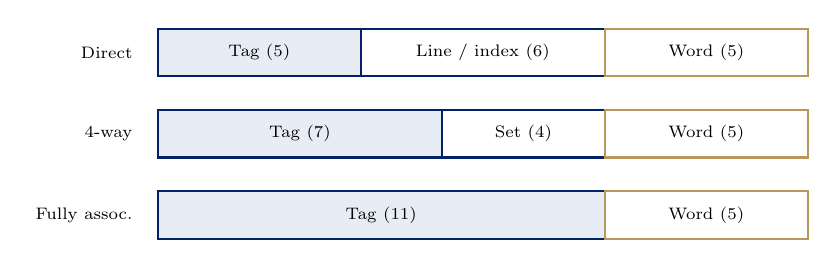
\begin{tikzpicture}[scale=0.86, transform shape,
        every node/.style={font=\scriptsize}]
      % ---- Row 1: direct mapped
      \draw[draw=primary-blue, thick, fill=light-bg] (0,2.05) rectangle (3.0,2.75);
      \draw[draw=primary-blue, thick, fill=white]    (3.0,2.05) rectangle (6.6,2.75);
      \draw[draw=primary-gold, thick, fill=white]    (6.6,2.05) rectangle (9.6,2.75);
      \node at (1.5,2.4) {Tag (5)};
      \node at (4.8,2.4) {Line / index (6)};
      \node at (8.1,2.4) {Word (5)};
      \node[anchor=east] at (-0.25,2.4) {Direct};
      % ---- Row 2: 4-way set associative
      \draw[draw=primary-blue, thick, fill=light-bg] (0,0.85) rectangle (4.2,1.55);
      \draw[draw=primary-blue, thick, fill=white]    (4.2,0.85) rectangle (6.6,1.55);
      \draw[draw=primary-gold, thick, fill=white]    (6.6,0.85) rectangle (9.6,1.55);
      \node at (2.1,1.2) {Tag (7)};
      \node at (5.4,1.2) {Set (4)};
      \node at (8.1,1.2) {Word (5)};
      \node[anchor=east] at (-0.25,1.2) {4-way};
      % ---- Row 3: fully associative
      \draw[draw=primary-blue, thick, fill=light-bg] (0,-0.35) rectangle (6.6,0.35);
      \draw[draw=primary-gold, thick, fill=white]    (6.6,-0.35) rectangle (9.6,0.35);
      \node at (3.3,0.0) {Tag (11)};
      \node at (8.1,0.0) {Word (5)};
      \node[anchor=east] at (-0.25,0.0) {Fully assoc.};
    \end{tikzpicture}
  \end{center}
  \textbf{What this diagram shows:} the word field never moves --- it is fixed
  by the block size alone. Everything to its left is a fixed budget of 11 bits
  that the index and tag \emph{share}. Less freedom in placement means a
  narrower tag; more freedom means a wider one.
\end{frame}

\begin{frame}{Direct Mapping: The Rule}
  \begin{block}{Direct mapping}
    Block $B$ of main memory may occupy \emph{exactly one} cache line:
    \[
      \text{line} \;=\; B \bmod L ,
      \qquad
      \text{tag} \;=\; \lfloor B / L \rfloor .
    \]
    The line number is read straight out of the address --- no search, no
    choice \cite[Fig.~5.7, PDF p.~190]{Stallings2015_computer_organization}.
  \end{block}
  \begin{itemize}
    \item Blocks $B$, $B+L$, $B+2L$, \dots\ all land on the same line. They are
      told apart \emph{only} by the tag.
    \item \good{Cheapest possible hardware}: one line decoder, one tag
      comparator.
    \item \bad{The cost}: two hot blocks that happen to be $L$ apart evict
      each other forever, no matter how empty the rest of the cache is.
  \end{itemize}
\end{frame}

\begin{frame}{How Blocks Collide on One Line}
  \begin{center}
    % Diagram: many-to-one mapping under direct mapping, drawn for a toy cache
    % of 4 lines so the modulo is visible. Only the two arrows that collide on
    % line 0 are drawn -- drawing all eight would produce crossing arrows with
    % no extra teaching value (tikz-measurement Pass 1, step 5).
    % Coordinates: (x, y). Memory blocks are 2.0-wide, 0.5-high boxes at x=0;
    % cache lines are 2.0-wide, 0.5-high boxes at x=6.0.
    %   Block 0 (0,3.5)  Block 1 (0,2.9)  Block 2 (0,2.3)  Block 3 (0,1.7)
    %   Block 4 (0,1.1)  Block 5 (0,0.5)  Block 6 (0,-0.1) Block 7 (0,-0.7)
    %   Line 0 (6.0,3.5) Line 1 (6.0,2.9) Line 2 (6.0,2.3) Line 3 (6.0,1.7)
    % P7a: block boxes span x -1.0..1.0, line boxes span x 5.0..7.0; both
    % arrows live entirely in the empty corridor x 1.0..5.0, crossing no box.
    % P7b: the horizontal arrow's label sits 0.35 above it; the diagonal's
    % label sits 0.35 below the diagonal's own y at that x (computed in the
    % comment on each \node below).
    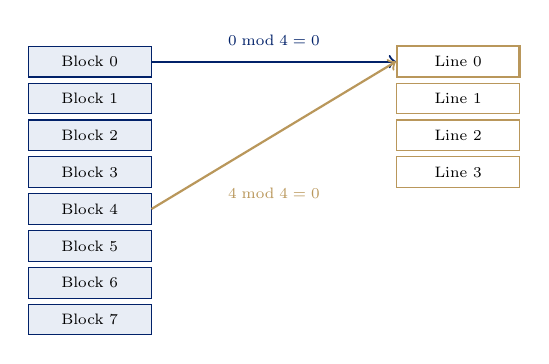
\begin{tikzpicture}[scale=0.78, transform shape,
        every node/.style={font=\scriptsize}]
      \node[draw=primary-blue, fill=light-bg, minimum width=2.0cm,
            minimum height=0.5cm] (B0) at (0,3.5)  {Block 0};
      \node[draw=primary-blue, fill=light-bg, minimum width=2.0cm,
            minimum height=0.5cm]       at (0,2.9)  {Block 1};
      \node[draw=primary-blue, fill=light-bg, minimum width=2.0cm,
            minimum height=0.5cm]       at (0,2.3)  {Block 2};
      \node[draw=primary-blue, fill=light-bg, minimum width=2.0cm,
            minimum height=0.5cm]       at (0,1.7)  {Block 3};
      \node[draw=primary-blue, fill=light-bg, minimum width=2.0cm,
            minimum height=0.5cm] (B4) at (0,1.1)  {Block 4};
      \node[draw=primary-blue, fill=light-bg, minimum width=2.0cm,
            minimum height=0.5cm]       at (0,0.5)  {Block 5};
      \node[draw=primary-blue, fill=light-bg, minimum width=2.0cm,
            minimum height=0.5cm]       at (0,-0.1) {Block 6};
      \node[draw=primary-blue, fill=light-bg, minimum width=2.0cm,
            minimum height=0.5cm]       at (0,-0.7) {Block 7};
      \node[draw=primary-gold, thick, fill=white, minimum width=2.0cm,
            minimum height=0.5cm] (L0) at (6.0,3.5) {Line 0};
      \node[draw=primary-gold, fill=white, minimum width=2.0cm,
            minimum height=0.5cm]       at (6.0,2.9) {Line 1};
      \node[draw=primary-gold, fill=white, minimum width=2.0cm,
            minimum height=0.5cm]       at (6.0,2.3) {Line 2};
      \node[draw=primary-gold, fill=white, minimum width=2.0cm,
            minimum height=0.5cm]       at (6.0,1.7) {Line 3};
      \draw[->, thick, primary-blue] (B0.east) -- (L0.west);
      \draw[->, thick, primary-gold] (B4.east) -- (L0.west);
      % horizontal arrow runs at y=3.5; label 0.35 above it
      \node[primary-blue] at (3.0,3.85) {$0 \bmod 4 = 0$};
      % diagonal descends to y=1.82 at the label's left edge (x=2.2), so the
      % label's top edge must stay below that: top 1.48 => centre 1.35,
      % leaving 0.35 clearance from the line across the whole label width
      \node[primary-gold] at (3.0,1.35) {$4 \bmod 4 = 0$};
    \end{tikzpicture}
  \end{center}
  \textbf{What this diagram shows (toy cache, $L=4$):} blocks 0, 4, 8, 12,
  \dots\ are all forced onto line 0. Only one may be resident at a time, and
  the tag records which. Blocks 1, 5, 9, \dots\ queue up for line 1, and so on.
\end{frame}

\begin{frame}{Direct-Mapped Hardware: One Comparator}
  \begin{center}
    % Diagram: direct-mapped lookup datapath. Address strip on top; the line
    % field indexes the cache array; the array emits the stored tag; ONE
    % comparator checks it against the address's tag field; result is hit/miss.
    % Coordinates: (x, y)
    %   Address strip: rectangles spanning y 4.2..4.9
    %       Tag  0.0..2.4 (centre x=1.2)
    %       Line 2.4..5.0 (centre x=3.7)
    %       Word 5.0..6.6 (centre x=5.8)
    %   Cache array box   centre (4.0, 1.9), w=6.0, h=2.6  -> x 1.0..7.0,   y 0.6..3.2
    %   Comparator box    centre (10.4,1.9), w=2.2, h=1.4  -> x 9.3..11.5,  y 1.2..2.6
    %   Hit/miss box      centre (14.2,1.9), w=2.0, h=0.9  -> x 13.2..15.2, y 1.45..2.35
    % P1: both multi-line boxed nodes carry text width (5.5cm / 1.9cm), so their
    %     text cannot grow past the declared minimum width.
    % P7a audit of every path:
    %   (3.7,4.2)->(3.7,3.2)  vertical in x=3.7: enters the array only at its
    %       top edge (y=3.2), a legitimate connection point. Clears the address
    %       strip (bottom y=4.2) exactly at its start point.
    %   (7.0,1.9)->(9.3,1.9)  horizontal in the empty corridor x 7.0..9.3.
    %   (1.2,4.9)->(1.2,5.8)->(10.4,5.8)->(10.4,2.6) : the y=5.8 leg is above
    %       every box (highest box top = 4.9); the x=10.4 drop is right of the
    %       array's east edge (7.0) and lands on the comparator's top edge.
    %   (11.5,1.9)->(13.2,1.9) horizontal in the empty corridor x 11.5..13.2.
    % P7b: each edge label sits >= 0.3 units (0.186 cm at scale 0.62) off its
    %      own line, never on it.
    % P7c: every unboxed label clears the nearest box edge by >= 0.25 units
    %      (0.155 cm at scale 0.62). Widths estimated at 0.161 units/char for
    %      \scriptsize (0.10 cm/char / 0.62 scale), per tikz-measurement Pass 2.
    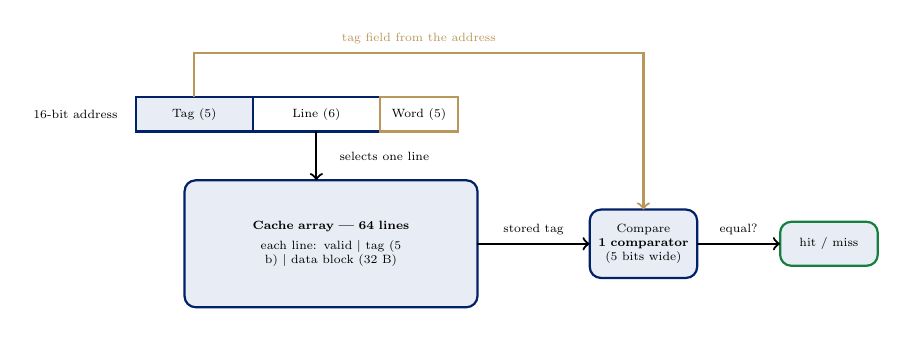
\begin{tikzpicture}[scale=0.62, transform shape,
        every node/.style={font=\scriptsize}]
      \draw[draw=primary-blue, thick, fill=light-bg] (0,4.2) rectangle (2.4,4.9);
      \draw[draw=primary-blue, thick, fill=white]    (2.4,4.2) rectangle (5.0,4.9);
      \draw[draw=primary-gold, thick, fill=white]    (5.0,4.2) rectangle (6.6,4.9);
      \node at (1.2,4.55) {Tag (5)};
      \node at (3.7,4.55) {Line (6)};
      \node at (5.8,4.55) {Word (5)};
      \node[anchor=east] at (-0.25,4.55) {16-bit address};
      \node[draw=primary-blue, thick, fill=light-bg, rounded corners,
            minimum width=6.0cm, minimum height=2.6cm, text width=5.5cm,
            align=center]
            (ARR) at (4.0,1.9)
            {\textbf{Cache array --- 64 lines}\\[0.12cm]
             each line: valid $\mid$ tag (5 b) $\mid$ data block (32 B)};
      \node[draw=primary-blue, thick, fill=light-bg, rounded corners,
            minimum width=2.2cm, minimum height=1.4cm, text width=1.9cm,
            align=center]
            (CMP) at (10.4,1.9) {Compare\\\textbf{1 comparator}\\(5 bits wide)};
      \node[draw=positive, thick, fill=light-bg, rounded corners,
            minimum width=2.0cm, minimum height=0.9cm, align=center]
            (HIT) at (14.2,1.9) {hit / miss};
      \draw[->, thick] (3.7,4.2) -- (3.7,3.2);
      \node[anchor=west] at (4.05,3.7) {selects one line};
      \draw[->, thick] (7.0,1.9) -- (9.3,1.9);
      \node at (8.15,2.20) {stored tag};
      \draw[->, thick, primary-gold] (1.2,4.9) -- (1.2,5.8) -- (10.4,5.8) -- (10.4,2.6);
      \node[primary-gold] at (5.80,6.10) {tag field from the address};
      \draw[->, thick] (11.5,1.9) -- (13.2,1.9);
      \node at (12.35,2.20) {equal?};
    \end{tikzpicture}
  \end{center}
  \textbf{What this diagram shows:} the line field is a \emph{decoder input},
  not something to search for. Only after the line is selected does a single
  comparison decide hit or miss.
\end{frame}

\begin{frame}{Direct Mapping, Worked: Deriving the Bit Widths}
  \begin{exampleblock}{System A: 64~KB memory, 2~KB cache, 32-byte blocks}
    Derive the width of every address field, step by step.
  \end{exampleblock}
  \begin{enumerate}
    \item Physical address width: $64\text{ KB} = 2^{16}$ bytes
      $\Rightarrow N = \key{16}$ bits.
    \item Word (offset) field: block $= 32 = 2^{5}$ bytes
      $\Rightarrow b = \key{5}$ bits.
    \item Number of lines: $L = 2\text{ KB} / 32\text{ B}
      = 2^{11}/2^{5} = 2^{6} = 64$
      $\Rightarrow$ line field $= \log_2 64 = \key{6}$ bits.
    \item Tag field $= N - \log_2 L - b = 16 - 6 - 5 = \key{5}$ bits.
  \end{enumerate}
  \vspace{0.15cm}
  \textbf{Check:} $5 + 6 + 5 = 16$ \good{\checkmark} --- the three fields must
  always re-sum to the full address width. If they do not, one of the four
  steps above is wrong.
\end{frame}

\begin{frame}{Direct Mapping, Worked: Tracing Address \texttt{0x3F8C}}
  \footnotesize
  \begin{exampleblock}{Which line does \texttt{0x3F8C} map to, and what is its tag?}
    $\texttt{0x3F8C} = 0011\,1111\,1000\,1100_2$. Slice it $5 \mid 6 \mid 5$
    from the left.
  \end{exampleblock}
  \vspace{-0.1cm}
  \begin{center}
  \begin{tabular}{@{}lll@{}}
    \toprule
    \textbf{Field} & \textbf{Bits} & \textbf{Value} \\
    \midrule
    Tag (5 b)  & \texttt{00111}  & $7$  \\
    Line (6 b) & \texttt{111100} & $60$ \\
    Word (5 b) & \texttt{01100}  & $12$ \\
    \bottomrule
  \end{tabular}
  \end{center}
  \vspace{0.15cm}
  \textbf{Now verify by arithmetic, not by bit-slicing:}
  \begin{itemize}
    \item $\texttt{0x3F8C} = 16268$; block $B = \lfloor 16268/32 \rfloor
      = 508$; offset $= 16268 - 508 \times 32 = 12$ \good{\checkmark}
    \item Line $= B \bmod L = 508 \bmod 64 = 508 - 448 = 60$
      \good{\checkmark}
    \item Tag $= \lfloor B/L \rfloor = \lfloor 508/64 \rfloor = 7$
      \good{\checkmark}
  \end{itemize}
  \muted{Two independent routes to the same answer. In an exam, do one and
  check with the other.}
\end{frame}

\begin{frame}{Direct Mapping's Weakness: Conflict Misses}
  \begin{block}{A two-block loop that defeats a 2~KB cache}
    A loop alternately touches address \texttt{0x0780} (block 60) and
    \texttt{0x0F80} (block 124). Both are in System A. What is the hit ratio?
  \end{block}
  \begin{itemize}
    \item $60 \bmod 64 = 60$ and $124 \bmod 64 = 60$ --- \key{both map to line
      60}, with tags $\lfloor 60/64 \rfloor = 0$ and $\lfloor 124/64 \rfloor
      = 1$.
    \item Every reference finds the \emph{other} block's tag in line 60, so
      every reference is a miss: hit ratio $= \key{0\%}$, while
      \key{63 of the 64 lines sit empty}.
    \item This is a \key{conflict (collision) miss} --- not a capacity
      problem, purely a placement-restriction problem.
    \item \good{Fix:} in a 2-way set-associative cache ($S = 64/2 = 32$ sets),
      $60 \bmod 32 = 28$ and $124 \bmod 32 = 28$ --- still the same set, but
      now the set has \key{two} ways, so both blocks stay resident and the hit
      ratio jumps to nearly \key{100\%}.
  \end{itemize}
\end{frame}

\begin{frame}{Fully Associative Mapping: The Rule}
  \begin{block}{Fully associative mapping}
    A block may be placed in \emph{any} cache line. There is no index field:
    the address splits into \key{tag} $\mid$ \key{word} only, and the tag is
    simply the block number
    \cite[Fig.~5.10, PDF p.~195]{Stallings2015_computer_organization}.
    \[
      \text{tag} = B = \lfloor \text{address} / 2^b \rfloor ,
      \qquad \text{tag width} = N - b .
    \]
  \end{block}
  \begin{itemize}
    \item \good{No conflict misses ever.} A block is evicted only when the
      cache is genuinely full --- so the only misses left are compulsory and
      capacity misses.
    \item \bad{Identification is now a search.} With no index to narrow the
      candidates, \emph{every} line's tag must be compared, simultaneously.
    \item That is what \key{content-addressable memory (CAM)} does: a memory
      searched by content rather than by address
      \cite[PDF pp.~193--194]{Stallings2015_computer_organization}.
  \end{itemize}
\end{frame}

\begin{frame}{Fully Associative, Worked: \texttt{0x3F8C} Again}
  \begin{exampleblock}{Same System A --- rederive from scratch}
    Only the block size changes the word field; everything else the tag
    absorbs.
  \end{exampleblock}
  \begin{enumerate}
    \item Word field $= b = \key{5}$ bits (unchanged --- 32-byte block).
    \item There is no index field, so tag $= N - b = 16 - 5 = \key{11}$ bits.
    \item Check: $11 + 5 = 16$ \good{\checkmark}
    \item Slice $\texttt{0x3F8C} = 0011\,1111\,1000\,1100_2$ as $11 \mid 5$:
      \begin{itemize}
        \item Tag $= \texttt{00111111100}_2 = 508$
        \item Word $= \texttt{01100}_2 = 12$
      \end{itemize}
    \item Verify: the tag \emph{is} the block number, and we computed
      $B = 508$ on the direct-mapping slide \good{\checkmark}
  \end{enumerate}
  \vspace{0.1cm}
  \muted{Answer to ``which line?'': \emph{any of the 64} --- that is precisely
  what fully associative means, and precisely why a replacement policy becomes
  necessary.}
\end{frame}

\begin{frame}{The Price of Full Associativity}
  \begin{block}{Count the hardware for System A}
    \begin{itemize}
      \item Comparators: \key{64}, one per line, each \key{11 bits} wide, all
        firing in parallel on every access.
      \item Tag storage: $64 \times 11 = \key{704}$ bits.
      \item Compare with direct mapping: \key{1} comparator of \key{5} bits,
        and $64 \times 5 = \key{320}$ tag bits.
    \end{itemize}
  \end{block}
  \begin{itemize}
    \item Full associativity costs \key{$2.2\times$ the tag storage} and
      \key{$64\times$ the comparators} --- and the comparator array is on the
      critical path, so it also costs \emph{access time}.
    \item Real caches with hundreds or thousands of lines cannot afford this.
      Hence the compromise on the next slide.
  \end{itemize}
\end{frame}

\begin{frame}{$k$-Way Set-Associative Mapping: The Rule}
  \begin{block}{$k$-way set associative mapping}
    Group the $L$ lines into $S = L/k$ \key{sets} of $k$ lines each. A block
    is mapped to \emph{one} set by index, and may occupy \emph{any} of the $k$
    lines (``ways'') inside it
    \cite[Fig.~5.13, PDF p.~200]{Stallings2015_computer_organization}:
    \[
      \text{set} = B \bmod S, \qquad
      \text{tag} = \lfloor B / S \rfloor, \qquad
      \text{tag width} = N - \log_2 S - b .
    \]
  \end{block}
  \begin{itemize}
    \item $k = 1$ gives $S = L$: that is exactly \key{direct mapping}.
    \item $k = L$ gives $S = 1$: that is exactly \key{fully associative
      mapping}.
    \item So set associativity is not a third idea --- it is the \emph{dial}
      between the other two, and $k = 2, 4, 8$ are the settings real designs
      use.
  \end{itemize}
\end{frame}

\begin{frame}{Set-Associative Hardware: $k$ Comparators}
  \begin{center}
    % Diagram: 4-way set-associative lookup. Deliberately the SAME skeleton as
    % the direct-mapped figure two slides earlier -- only the comparator count
    % and the width of the index field change. Keeping the layout identical is
    % the pedagogical point (tikz-measurement Pass 0, cross-slide consistency).
    % Coordinates: (x, y)
    %   Address strip: rectangles spanning y 4.2..4.9
    %       Tag  0.0..3.0 (centre x=1.5)
    %       Set  3.0..4.8 (centre x=3.9)
    %       Word 4.8..6.6 (centre x=5.7)
    %   Set array box     centre (4.0, 1.9), w=6.0, h=2.6  -> x 1.0..7.0, y 0.6..3.2
    %   Comparator box    centre (10.0,1.9), w=2.2, h=2.6  -> x 8.9..11.1, y 0.6..3.2
    %   Hit-OR box        centre (13.4,1.9), w=2.0, h=0.9  -> x 12.4..14.4, y 1.45..2.35
    % P7a audit of every path:
    %   (3.9,4.2)->(3.9,3.2) : vertical, meets the array only at its top edge.
    %   four horizontals at y = 2.8, 2.2, 1.6, 1.0 from x=7.0 to x=8.9 : all
    %       lie in the empty corridor between the array's east edge (7.0) and
    %       the comparator block's west edge (8.9); all four y-values are
    %       inside both boxes' vertical spans, so each meets a box edge only.
    %   (1.5,4.9)->(1.5,5.8)->(10.0,5.8)->(10.0,3.2) : the y=5.8 leg is above
    %       every box; the x=10.0 drop is right of the array (east edge 7.0)
    %       and lands on the comparator block's top edge.
    %   (11.1,1.9)->(12.4,1.9) : empty corridor.
    % P7b: "4 stored tags" sits at (7.95,3.15), 0.35 above the topmost of the
    %       four horizontals (y=2.8) and outside both boxes in x.
    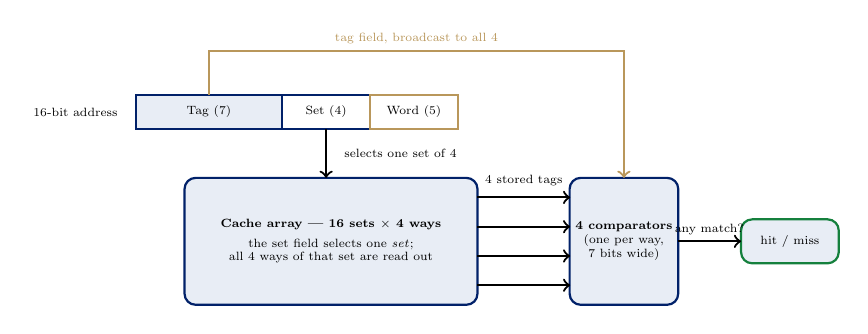
\begin{tikzpicture}[scale=0.62, transform shape,
        every node/.style={font=\scriptsize}]
      \draw[draw=primary-blue, thick, fill=light-bg] (0,4.2) rectangle (3.0,4.9);
      \draw[draw=primary-blue, thick, fill=white]    (3.0,4.2) rectangle (4.8,4.9);
      \draw[draw=primary-gold, thick, fill=white]    (4.8,4.2) rectangle (6.6,4.9);
      \node at (1.5,4.55) {Tag (7)};
      \node at (3.9,4.55) {Set (4)};
      \node at (5.7,4.55) {Word (5)};
      \node[anchor=east] at (-0.25,4.55) {16-bit address};
      \node[draw=primary-blue, thick, fill=light-bg, rounded corners,
            minimum width=6.0cm, minimum height=2.6cm, align=center]
            (ARR) at (4.0,1.9)
            {\textbf{Cache array --- 16 sets $\times$ 4 ways}\\[0.12cm]
             the set field selects one \emph{set};\\
             all 4 ways of that set are read out};
      \node[draw=primary-blue, thick, fill=light-bg, rounded corners,
            minimum width=2.2cm, minimum height=2.6cm, align=center]
            (CMP) at (10.0,1.9) {\textbf{4 comparators}\\(one per way,\\7 bits wide)};
      \node[draw=positive, thick, fill=light-bg, rounded corners,
            minimum width=2.0cm, minimum height=0.9cm, align=center]
            (HIT) at (13.4,1.9) {hit / miss};
      \draw[->, thick] (3.9,4.2) -- (3.9,3.2);
      \node[anchor=west] at (4.15,3.7) {selects one set of 4};
      \draw[->, thick] (7.0,2.8) -- (8.9,2.8);
      \draw[->, thick] (7.0,2.2) -- (8.9,2.2);
      \draw[->, thick] (7.0,1.6) -- (8.9,1.6);
      \draw[->, thick] (7.0,1.0) -- (8.9,1.0);
      \node at (7.95,3.15) {4 stored tags};
      \draw[->, thick, primary-gold] (1.5,4.9) -- (1.5,5.8) -- (10.0,5.8) -- (10.0,3.2);
      \node[primary-gold] at (5.75,6.05) {tag field, broadcast to all 4};
      \draw[->, thick] (11.1,1.9) -- (12.4,1.9);
      \node at (11.75,2.15) {any match?};
    \end{tikzpicture}
  \end{center}
  \textbf{Compare with the direct-mapped figure:} identical skeleton, one
  comparator becomes $k$, and two bits move from the index field into the tag.
\end{frame}

\begin{frame}{4-Way Set Associative, Worked: Bit Widths}
  \begin{exampleblock}{System A again, now organised 4-way}
    64~KB memory, 2~KB cache, 32-byte blocks, $k = 4$.
  \end{exampleblock}
  \begin{enumerate}
    \item Address width $N = \key{16}$; word field $b = \key{5}$ (both
      unchanged --- neither depends on associativity).
    \item Lines $L = 64$ (unchanged --- cache size and block size alone fix
      it).
    \item Number of sets $S = L/k = 64/4 = \key{16}$
      $\Rightarrow$ set field $= \log_2 16 = \key{4}$ bits.
    \item Tag $= N - \log_2 S - b = 16 - 4 - 5 = \key{7}$ bits.
    \item Check: $7 + 4 + 5 = 16$ \good{\checkmark}
  \end{enumerate}
  \vspace{0.1cm}
  \muted{Notice what moved: going from direct ($k{=}1$) to 4-way, the index
  lost 2 bits ($6 \to 4$) and the tag gained exactly those 2 ($5 \to 7$).
  Doubling $k$ always trades one index bit for one tag bit.}
\end{frame}

\begin{frame}{4-Way Set Associative, Worked: Tracing \texttt{0x3F8C}}
  \footnotesize
  \begin{exampleblock}{Which \emph{set} does \texttt{0x3F8C} map to, and what is its tag?}
    $\texttt{0x3F8C} = 0011\,1111\,1000\,1100_2$, sliced $7 \mid 4 \mid 5$.
  \end{exampleblock}
  \vspace{-0.1cm}
  \begin{center}
  \begin{tabular}{@{}lll@{}}
    \toprule
    \textbf{Field} & \textbf{Bits} & \textbf{Value} \\
    \midrule
    Tag (7 b)  & \texttt{0011111} & $31$ \\
    Set (4 b)  & \texttt{1100}    & $12$ \\
    Word (5 b) & \texttt{01100}   & $12$ \\
    \bottomrule
  \end{tabular}
  \end{center}
  \vspace{0.15cm}
  \textbf{Arithmetic cross-check} (block $B = 508$, as before):
  \begin{itemize}
    \item Set $= B \bmod S = 508 \bmod 16 = 508 - 496 = 12$ \good{\checkmark}
    \item Tag $= \lfloor B/S \rfloor = \lfloor 508/16 \rfloor = 31$
      \good{\checkmark}
    \item Word offset $= 12$, unchanged in all three schemes \good{\checkmark}
  \end{itemize}
  \key{The answer to ``which line?''} is now: \emph{any of the 4 ways of set
  12} --- which is exactly where a replacement policy is finally needed.
\end{frame}

\begin{frame}{Hardware Cost, Counted}
  \footnotesize
  \begin{center}
  \begin{tabular}{@{}lccccc@{}}
    \toprule
    \textbf{Organisation} & \textbf{Sets $S$} & \textbf{Index bits} &
    \textbf{Tag bits} & \textbf{Comparators} & \textbf{Total tag storage} \\
    \midrule
    Direct ($k{=}1$)      & 64 & 6 & 5  & 1  & $64\times5 = 320$ b \\
    2-way                 & 32 & 5 & 6  & 2  & $64\times6 = 384$ b \\
    4-way                 & 16 & 4 & 7  & 4  & $64\times7 = 448$ b \\
    8-way                 & 8  & 3 & 8  & 8  & $64\times8 = 512$ b \\
    Fully associative     & 1  & 0 & 11 & 64 & $64\times11 = 704$ b \\
    \bottomrule
  \end{tabular}
  \end{center}
  \vspace{0.25cm}
  \normalsize
  \begin{itemize}
    \item All rows are System A --- same 64 lines, same 32-byte blocks. Only
      the \emph{grouping} changes.
    \item Comparator count \key{doubles} with every doubling of $k$; tag
      storage grows only \key{one bit per line}. The comparators, not the tag
      bits, are what make full associativity unaffordable.
    \item \muted{Add one valid bit per line throughout (and one dirty bit under
      write-back) --- constant across all rows, so it does not change the
      comparison.}
  \end{itemize}
\end{frame}

\begin{frame}{The Three Mapping Schemes, Head to Head}
  \tiny
  \begin{center}
  \begin{tabular}{@{}lllll@{}}
    \toprule
    & \textbf{Direct} & \textbf{$k$-way set associative} & \textbf{Fully associative} \\
    \midrule
    Address split & tag $\mid$ line $\mid$ word & tag $\mid$ set $\mid$ word & tag $\mid$ word \\
    Index width & $\log_2 L$ & $\log_2 (L/k)$ & $0$ \\
    Tag width & $N - \log_2 L - b$ & $N - \log_2 (L/k) - b$ & $N - b$ \\
    Placement rule & line $= B \bmod L$ & set $= B \bmod (L/k)$ & anywhere \\
    Candidate lines & 1 & $k$ & all $L$ \\
    Comparators & 1 & $k$ & $L$ \\
    Replacement policy & \bad{none needed} & needed, within the set & needed, over the whole cache \\
    Conflict misses & \bad{severe} & \muted{reduced, roughly as $k$ grows} & \good{none} \\
    Search hardware & decoder only & decoder $+$ $k$ comparators & full CAM \\
    Access time & \good{fastest} & \muted{intermediate} & \bad{slowest} \\
    Typical use & simple / large L2--L3 & \good{L1 and L2 in practice} & TLBs, small victim caches \\
    \bottomrule
  \end{tabular}
  \end{center}
  \vspace{0.3cm}
  \normalsize
  \key{One dial, two end-stops.} $k = 1$ and $k = L$ are the extremes of the
  same formula; every real design lives somewhere in between
  \cite[\S5.2, PDF pp.~187--203]{Stallings2015_computer_organization}.
\end{frame}

\begin{frame}{Socratic Check: Choosing an Organisation}
  \begin{alertblock}{Question}
    An L1 data cache must answer in one CPU cycle. A last-level L3 cache may
    take twenty cycles but must not waste its (large) capacity. Which
    associativity would you pick for each, and why?
  \end{alertblock}
  \begin{itemize}
    \item \key{L1}: low associativity (2- or 4-way). The comparator array is
      on the critical path, and a 1-cycle budget cannot afford 64 parallel
      comparisons. Some conflict misses are the accepted price.
    \item \key{L3}: higher associativity (8- or 16-way). Latency is already
      large, so a wider comparator array is affordable --- and with a big
      cache, wasting capacity to conflicts is the more expensive mistake.
    \item \muted{The general rule: associativity buys hit ratio and costs
      access time. Spend it where access time is not the binding constraint.}
  \end{itemize}
\end{frame}

\transitionslide{Act 5: the set is full and a new block arrives. Which resident block dies?}

% =============================================================================
% ACT 5 --- REPLACEMENT ALGORITHMS
% =============================================================================
\section{Replacement Algorithms}

\begin{frame}{When Is There Anything to Decide?}
  \begin{block}{Replacement exists only where placement offers a choice}
    \begin{itemize}
      \item \key{Direct mapping needs no replacement algorithm at all.} A
        block has exactly one legal line; if that line is occupied, the
        occupant is evicted. There is no decision to make, so there is no
        policy to implement
        \cite[\S5.2 Replacement Algorithms, PDF p.~203]{Stallings2015_computer_organization}.
      \item \key{Fully associative}: the victim is chosen among \emph{all}
        $L$ lines.
      \item \key{$k$-way set associative}: the victim is chosen among the
        \emph{$k$ lines of the target set} --- never across sets.
    \end{itemize}
  \end{block}
  \begin{itemize}
    \item To be useful at cache speed, a policy must be implementable
      \emph{entirely in hardware} --- no software bookkeeping, no sorting.
      That constraint eliminates many policies that look good on paper.
  \end{itemize}
\end{frame}

\begin{frame}{Five Policies}
  \footnotesize
  \begin{itemize}
    \item \key{LRU (Least Recently Used)} --- evict the line unreferenced for
      longest. Exploits temporal locality directly; the most popular policy in
      practice
      \cite[\S5.2, PDF p.~203]{Stallings2015_computer_organization}.
    \item \key{FIFO (First In, First Out)} --- evict the line resident
      longest, regardless of use. Implementable as a round-robin/circular
      buffer.
    \item \key{LFU (Least Frequently Used)} --- evict the line with the
      smallest reference count.
    \item \key{Random} --- evict a line chosen at random. Simulation studies
      report only slightly inferior performance to the usage-based algorithms
      \cite[\S5.2, PDF p.~203]{Stallings2015_computer_organization}.
    \item \key{OPT (Optimal / Belady's MIN)} --- evict the line whose
      \emph{next} reference is furthest in the future.
  \end{itemize}
  \vspace{0.15cm}
  \begin{alertblock}{Sourcing note --- read this carefully}
    The first four are Stallings' four cache replacement algorithms. \key{OPT
    is not in that text at all}; it is presented here as \emph{standard
    general treatment, with no page citation}. OPT is also \key{unimplementable}
    --- it requires knowing the future. Its role is as a \emph{benchmark}: no
    real policy can beat it, so it bounds how much a better policy could
    possibly gain.
  \end{alertblock}
\end{frame}

\begin{frame}{The Common Reference String}
  \begin{exampleblock}{One experiment, five policies}
    A \key{fully associative} cache with \key{3 lines}, initially empty,
    receives this stream of \emph{block numbers}:
    \[
      7,\;0,\;1,\;2,\;0,\;3,\;0,\;4,\;2,\;3,\;0,\;3,\;2
      \qquad (13 \text{ references})
    \]
  \end{exampleblock}
  \begin{itemize}
    \item Three lines makes every eviction a genuine three-way choice, so the
      policies actually diverge --- which is the point.
    \item In the traces that follow, each column is one reference. The three
      rows are the three cache lines (slots), \texttt{M} marks a miss and
      \good{\texttt{H}} a hit.
    \item The first three references are \key{compulsory misses}: an empty
      cache must miss on first touch, whatever the policy. Every policy scores
      at least 3 misses here, so only the remaining 10 references separate
      them.
  \end{itemize}
\end{frame}

\begin{frame}{Trace 1 --- FIFO}
  \tiny
  \begin{center}
  \begin{tabular}{@{}l*{13}{c}@{}}
    \toprule
    Reference & 7 & 0 & 1 & 2 & 0 & 3 & 0 & 4 & 2 & 3 & 0 & 3 & 2 \\
    \midrule
    Slot 0 & 7 & 7 & 7 & \textbf{2} & 2 & 2 & 2 & \textbf{4} & 4 & 4 & \textbf{0} & 0 & 0 \\
    Slot 1 & -- & 0 & 0 & 0 & 0 & \textbf{3} & 3 & 3 & \textbf{2} & 2 & 2 & 2 & 2 \\
    Slot 2 & -- & -- & 1 & 1 & 1 & 1 & \textbf{0} & 0 & 0 & \textbf{3} & 3 & 3 & 3 \\
    \midrule
    Hit/Miss & M & M & M & M & \good{H} & M & M & M & M & M & M & \good{H} & \good{H} \\
    \bottomrule
  \end{tabular}
  \end{center}
  \vspace{0.3cm}
  \normalsize
  \begin{itemize}
    \item Victims are taken in strict round-robin order: slot 0, 1, 2, 0,
      \dots\ --- FIFO never looks at whether a block is being used.
    \item Reference 7 is the tell: block 0 was referenced only two steps
      earlier, yet FIFO evicts it because it happened to arrive early.
    \item \key{Result: 3 hits, 10 misses} --- hit ratio $3/13 = 23.1\%$.
  \end{itemize}
\end{frame}

\begin{frame}{Trace 2 --- LRU}
  \tiny
  \begin{center}
  \begin{tabular}{@{}l*{13}{c}@{}}
    \toprule
    Reference & 7 & 0 & 1 & 2 & 0 & 3 & 0 & 4 & 2 & 3 & 0 & 3 & 2 \\
    \midrule
    Slot 0 & 7 & 7 & 7 & \textbf{2} & 2 & 2 & 2 & \textbf{4} & 4 & 4 & \textbf{0} & 0 & 0 \\
    Slot 1 & -- & 0 & 0 & 0 & 0 & 0 & 0 & 0 & 0 & \textbf{3} & 3 & 3 & 3 \\
    Slot 2 & -- & -- & 1 & 1 & 1 & \textbf{3} & 3 & 3 & \textbf{2} & 2 & 2 & 2 & 2 \\
    \midrule
    Hit/Miss & M & M & M & M & \good{H} & M & \good{H} & M & M & M & M & \good{H} & \good{H} \\
    \bottomrule
  \end{tabular}
  \end{center}
  \vspace{0.3cm}
  \normalsize
  \begin{itemize}
    \item At reference 6, the resident blocks are $\{2,0,1\}$ with block 1
      unreferenced since step 3 --- so LRU evicts \emph{block 1}, where FIFO
      evicted block 0.
    \item That single better decision buys the extra hit at reference 7.
    \item \key{Result: 4 hits, 9 misses} --- hit ratio $4/13 = 30.8\%$,
      beating FIFO.
  \end{itemize}
\end{frame}

\begin{frame}{Trace 3 --- LFU}
  \tiny
  \begin{center}
  \begin{tabular}{@{}l*{13}{c}@{}}
    \toprule
    Reference & 7 & 0 & 1 & 2 & 0 & 3 & 0 & 4 & 2 & 3 & 0 & 3 & 2 \\
    \midrule
    Slot 0 & 7 & 7 & 7 & \textbf{2} & 2 & 2 & 2 & \textbf{4} & 4 & \textbf{3} & 3 & 3 & 3 \\
    Slot 1 & -- & 0 & 0 & 0 & 0 & 0 & 0 & 0 & 0 & 0 & 0 & 0 & 0 \\
    Slot 2 & -- & -- & 1 & 1 & 1 & \textbf{3} & 3 & 3 & \textbf{2} & 2 & 2 & 2 & 2 \\
    \midrule
    Count of 0 & -- & 1 & 1 & 1 & 2 & 2 & 3 & 3 & 3 & 3 & 4 & 4 & 4 \\
    \midrule
    Hit/Miss & M & M & M & M & \good{H} & M & \good{H} & M & M & M & \good{H} & \good{H} & \good{H} \\
    \bottomrule
  \end{tabular}
  \end{center}
  \vspace{0.25cm}
  \normalsize
  \begin{itemize}
    \item Ties in count are broken by age (oldest first). Block 0's count
      climbs to 3 by reference 7, so LFU \key{protects it} at reference 8 ---
      where LRU evicted it at reference 10.
    \item \key{Result: 5 hits, 8 misses} --- hit ratio $5/13 = 38.5\%$, the
      best of the four implementable policies on \emph{this} string.
    \item \muted{Do not over-generalise: LFU's weakness is stale popularity ---
      a block referenced heavily long ago keeps a high count and refuses to
      leave. On a different string LRU wins.}
  \end{itemize}
\end{frame}

\begin{frame}{Trace 4 --- Random (One Particular Run)}
  \tiny
  \begin{center}
  \begin{tabular}{@{}l*{13}{c}@{}}
    \toprule
    Reference & 7 & 0 & 1 & 2 & 0 & 3 & 0 & 4 & 2 & 3 & 0 & 3 & 2 \\
    \midrule
    Slot 0 & 7 & 7 & 7 & 7 & \textbf{0} & \textbf{3} & 3 & \textbf{4} & 4 & 4 & \textbf{0} & 0 & 0 \\
    Slot 1 & -- & 0 & 0 & \textbf{2} & 2 & 2 & 2 & 2 & 2 & 2 & 2 & 2 & 2 \\
    Slot 2 & -- & -- & 1 & 1 & 1 & 1 & \textbf{0} & 0 & 0 & \textbf{3} & 3 & 3 & 3 \\
    \midrule
    Hit/Miss & M & M & M & M & M & M & M & M & \good{H} & M & M & \good{H} & \good{H} \\
    \bottomrule
  \end{tabular}
  \end{center}
  \vspace{0.3cm}
  \normalsize
  \begin{itemize}
    \item \key{Result of this run: 3 hits, 10 misses} --- hit ratio $23.1\%$.
    \item \bad{This number is not reproducible.} A different sequence of random
      victims gives a different count; only the \emph{expected} hit ratio over
      many runs is a property of the policy.
    \item So why use it? It needs \key{zero bookkeeping hardware} --- no
      counters, no recency list, no age bits --- and simulation studies find it
      only slightly inferior to the usage-based algorithms
      \cite[\S5.2, PDF p.~203]{Stallings2015_computer_organization}.
  \end{itemize}
\end{frame}

\begin{frame}{Trace 5 --- OPT (the Unattainable Benchmark)}
  \tiny
  \begin{center}
  \begin{tabular}{@{}l*{13}{c}@{}}
    \toprule
    Reference & 7 & 0 & 1 & 2 & 0 & 3 & 0 & 4 & 2 & 3 & 0 & 3 & 2 \\
    \midrule
    Slot 0 & 7 & 7 & 7 & \textbf{2} & 2 & 2 & 2 & 2 & 2 & 2 & 2 & 2 & 2 \\
    Slot 1 & -- & 0 & 0 & 0 & 0 & 0 & 0 & \textbf{4} & 4 & 4 & \textbf{0} & 0 & 0 \\
    Slot 2 & -- & -- & 1 & 1 & 1 & \textbf{3} & 3 & 3 & 3 & 3 & 3 & 3 & 3 \\
    \midrule
    Hit/Miss & M & M & M & M & \good{H} & M & \good{H} & M & \good{H} & \good{H} & M & \good{H} & \good{H} \\
    \bottomrule
  \end{tabular}
  \end{center}
  \vspace{0.25cm}
  \normalsize
  \begin{itemize}
    \item How the decisions are made: at reference 8 the residents are
      $\{2,0,3\}$; their next uses are block 2 at step 9, block 3 at step 10,
      block 0 at step 11. \key{Block 0 is used furthest away, so block 0 is
      evicted} --- the opposite of what LFU chose.
    \item \key{Result: 6 hits, 7 misses} --- hit ratio $6/13 = 46.2\%$.
    \item \muted{Standard general treatment --- not from Stallings, which does
      not cover OPT. Use it as a yardstick, never as a design.}
  \end{itemize}
\end{frame}

\begin{frame}{The Five Policies, Same Input, Different Outcomes}
  \footnotesize
  \begin{center}
  \begin{tabular}{@{}lccll@{}}
    \toprule
    \textbf{Policy} & \textbf{Hits} & \textbf{Misses} & \textbf{Hit ratio} & \textbf{What it tracks} \\
    \midrule
    OPT (benchmark)     & 6 & 7  & 46.2\% & the future (unimplementable) \\
    LFU                 & 5 & 8  & 38.5\% & a reference counter per line \\
    LRU                 & 4 & 9  & 30.8\% & recency order of the lines \\
    FIFO                & 3 & 10 & 23.1\% & load order only \\
    Random (this run)   & 3 & 10 & 23.1\% & nothing \\
    \bottomrule
  \end{tabular}
  \end{center}
  \vspace{0.3cm}
  \normalsize
  \begin{itemize}
    \item Identical input, identical cache, \key{a 2$\times$ spread in hit
      ratio} --- the policy is not a detail.
    \item OPT's $46.2\%$ is the ceiling: no implementable policy on this string
      can do better, so LFU's $38.5\%$ leaves at most $7.7$ percentage points
      on the table.
    \item \muted{One string proves nothing about policies in general. It proves
      that policies diverge --- which is why real designs are chosen by
      simulation over real traces, not by argument.}
  \end{itemize}
\end{frame}

\begin{frame}{Belady's Anomaly: More Cache, More Misses}
  \begin{block}{The claim that ought to be impossible}
    Under \key{FIFO}, \emph{increasing} the number of cache lines can
    \emph{increase} the number of misses on the same reference string. This is
    \key{Belady's anomaly}.
  \end{block}
  \tiny
  \textbf{Reference string:} $1,2,3,4,1,2,5,1,2,3,4,5$ \quad---\quad
  \textbf{FIFO with 3 lines:}
  \begin{center}
  \begin{tabular}{@{}l*{12}{c}@{}}
    \toprule
    Reference & 1 & 2 & 3 & 4 & 1 & 2 & 5 & 1 & 2 & 3 & 4 & 5 \\
    \midrule
    Slot 0 & 1 & 1 & 1 & \textbf{4} & 4 & 4 & \textbf{5} & 5 & 5 & 5 & 5 & 5 \\
    Slot 1 & -- & 2 & 2 & 2 & \textbf{1} & 1 & 1 & 1 & 1 & \textbf{3} & 3 & 3 \\
    Slot 2 & -- & -- & 3 & 3 & 3 & \textbf{2} & 2 & 2 & 2 & 2 & \textbf{4} & 4 \\
    \midrule
    Hit/Miss & M & M & M & M & M & M & M & \good{H} & \good{H} & M & M & \good{H} \\
    \bottomrule
  \end{tabular}
  \end{center}
  \normalsize
  \vspace{0.2cm}
  \key{3 lines $\Rightarrow$ 9 misses, 3 hits.} Now give the cache one more
  line and count again on the next slide.
  \vspace{0.1cm}
  \muted{\scriptsize Standard general treatment: Belady's anomaly appears
  nowhere in this course's Stallings text, so no page is cited for it.}
\end{frame}

\begin{frame}{Belady's Anomaly: The Punchline}
  \tiny
  \textbf{Same string} $1,2,3,4,1,2,5,1,2,3,4,5$ \quad---\quad
  \textbf{FIFO with 4 lines:}
  \begin{center}
  \begin{tabular}{@{}l*{12}{c}@{}}
    \toprule
    Reference & 1 & 2 & 3 & 4 & 1 & 2 & 5 & 1 & 2 & 3 & 4 & 5 \\
    \midrule
    Slot 0 & 1 & 1 & 1 & 1 & 1 & 1 & \textbf{5} & 5 & 5 & 5 & \textbf{4} & 4 \\
    Slot 1 & -- & 2 & 2 & 2 & 2 & 2 & 2 & \textbf{1} & 1 & 1 & 1 & \textbf{5} \\
    Slot 2 & -- & -- & 3 & 3 & 3 & 3 & 3 & 3 & \textbf{2} & 2 & 2 & 2 \\
    Slot 3 & -- & -- & -- & 4 & 4 & 4 & 4 & 4 & 4 & \textbf{3} & 3 & 3 \\
    \midrule
    Hit/Miss & M & M & M & M & \good{H} & \good{H} & M & M & M & M & M & M \\
    \bottomrule
  \end{tabular}
  \end{center}
  \normalsize
  \vspace{0.25cm}
  \begin{alertblock}{The result}
    \key{3 lines: 9 misses. \quad 4 lines: 10 misses.} A \emph{bigger} cache
    performed \emph{worse} on the identical reference string.
  \end{alertblock}
  \begin{itemize}
    \item \key{LRU and OPT are immune.} They are \emph{stack algorithms}: the
      set of blocks held with $n$ lines is always a subset of the set held with
      $n+1$ lines, so extra capacity can never remove a block that would
      otherwise have hit.
    \item FIFO has no such property --- adding a line changes the eviction
      order itself, not just its depth.
  \end{itemize}
\end{frame}

\begin{frame}{Implementing These Policies in Hardware}
  \scriptsize
  \begin{block}{Each policy is only as good as the hardware it needs}
    \begin{itemize}
      \item \key{LRU, two-way set associative} --- one \key{USE bit} per set.
        Referencing way 0 sets the bit to 0, referencing way 1 sets it to 1;
        the victim is the way the bit does \emph{not} point at. One bit per
        set, total \cite[\S5.2, PDF p.~203]{Stallings2015_computer_organization}.
      \item \key{LRU, fully associative} --- maintain an \key{index list} of
        all $L$ lines in recency order. A reference moves that line to the
        front; the victim is the tail. Correct, but the list must be reordered
        on \emph{every} access, which is why exact LRU is rare beyond small
        associativities
        \cite[\S5.2, PDF p.~203]{Stallings2015_computer_organization}.
      \item \key{FIFO} --- a \key{circular buffer} (round-robin pointer) per
        set. Advance the pointer on each replacement; no update at all on a
        hit. $\lceil \log_2 k \rceil$ bits per set.
      \item \key{LFU} --- a \key{reference counter} per line, incremented on
        every access to that line; the victim is the minimum. Costs a counter
        and a comparison tree per set, and needs periodic ageing to stop stale
        counts dominating.
      \item \key{Random} --- a free-running counter or LFSR shared by the whole
        cache. \key{No per-line state whatsoever}, which is exactly its appeal.
    \end{itemize}
  \end{block}
  \key{The pattern}: cost rises with how much history the policy remembers.
  Random remembers nothing; exact LRU remembers everything.
\end{frame}

\begin{frame}{Socratic Check: Why Is 2-Way LRU So Cheap?}
  \begin{alertblock}{Question}
    Exact LRU over 64 fully associative lines needs a 64-entry ordered list.
    Exact LRU over a 2-way set needs \emph{one bit}. Where did the cost go?
  \end{alertblock}
  \begin{itemize}
    \item Recency order over $n$ items is a \emph{permutation}: there are $n!$
      of them, needing $\lceil \log_2 n! \rceil$ bits. For $n = 2$ that is
      $\lceil \log_2 2 \rceil = 1$ bit; for $n = 64$ it is roughly
      \key{296 bits per set}.
    \item So associativity does not merely cost comparators (Act 4) --- it
      costs \key{replacement bookkeeping too}, and that cost grows far faster
      than linearly.
    \item \muted{This is why real 8- and 16-way caches use \emph{pseudo}-LRU
      (a small tree of bits that approximates recency) rather than exact LRU.}
  \end{itemize}
\end{frame}

\transitionslide{Act 6: put a number on all of it --- hit ratio, AMAT, and two cache levels.}

% =============================================================================
% ACT 6 --- QUANTITATIVE CACHE PERFORMANCE
% =============================================================================
\section{Cache Performance}

\begin{frame}{Hit Ratio, Miss Ratio, and AMAT}
  \begin{block}{The three definitions everything else is built from}
    For $n$ memory references of which $n_h$ hit in the cache:
    \[
      H = \frac{n_h}{n}, \qquad
      \text{miss ratio} = 1 - H,
    \]
    \[
      \text{AMAT} \;=\; T_{\text{hit}} \;+\; (1-H)\times T_{\text{miss penalty}} .
    \]
    AMAT is the \key{average memory access time} seen by the CPU
    \cite[\S5.3, p.~397]{PattersonHennessy2017_computer_organization_design}.
  \end{block}
  \begin{itemize}
    \item \key{Reconciling the two textbook forms.} Act 1 wrote
      $T_{\text{avg}} = H T_1 + (1-H)(T_1+T_2)$. Expanding gives
      $T_1 + (1-H)T_2$ --- identical to AMAT with
      $T_{\text{hit}} = T_1$ and miss penalty $= T_2$.
    \item The trap: a miss penalty is the \key{extra} time \emph{beyond} the
      hit time, because the hit time is paid on every access, hit or miss.
      Adding it twice is the single most common arithmetic error here.
  \end{itemize}
\end{frame}

\begin{frame}{Worked Example: AMAT from a Reference Count}
  \begin{exampleblock}{The setup}
    A program makes 1000 memory references; 940 are found in the cache. Cache
    access time is 2~ns and a miss costs a further 80~ns to fetch the block
    from main memory. Find the hit ratio, miss ratio and AMAT.
  \end{exampleblock}
  \begin{itemize}
    \item Hit ratio $H = 940/1000 = \key{0.94}$; miss ratio
      $= 1 - 0.94 = \key{0.06}$.
    \item $\text{AMAT} = 2 + 0.06 \times 80 = 2 + 4.8 = \key{6.8}$~ns.
    \item Cross-check with the Act 1 form:
      $0.94 \times 2 + 0.06 \times (2 + 80) = 1.88 + 4.92 = 6.8$~ns
      \good{\checkmark}
    \item \muted{Sanity test on any AMAT answer: it must lie strictly between
      the hit time (2~ns) and the full miss time (82~ns). $6.8$ does.}
  \end{itemize}
\end{frame}

\begin{frame}{Two Cache Levels: Two Access Models}
  \footnotesize
  \begin{block}{The distinction that decides the arithmetic}
    With an L1 cache (time $t_1$, hit ratio $h_1$), an L2 cache (time $t_2$,
    \emph{local} hit ratio $h_2$ measured over L1 misses only), and main memory
    (time $t_m$):
    \begin{itemize}
      \item \key{Hierarchical (sequential) access} --- each level is searched
        only after the one above it misses, so its time \emph{adds}:
        \[ T = h_1 t_1 + (1-h_1)h_2(t_1+t_2) + (1-h_1)(1-h_2)(t_1+t_2+t_m). \]
      \item \key{Simultaneous access} --- levels are probed in parallel, so
        only the level that answers contributes:
        \[ T = h_1 t_1 + (1-h_1)h_2\,t_2 + (1-h_1)(1-h_2)\,t_m. \]
    \end{itemize}
  \end{block}
  \muted{Always read the question for which model is intended. Unless a problem
  says otherwise, assume hierarchical --- it is what real multi-level caches do
  \cite[\S5.2 Number of Caches, PDF pp.~205--208]{Stallings2015_computer_organization}.}
\end{frame}

\begin{frame}{Worked Example: Effective Access Time, Hierarchical}
  \begin{exampleblock}{The setup}
    $t_1 = 1$~ns with $h_1 = 0.95$; $t_2 = 10$~ns with local $h_2 = 0.90$;
    main memory $t_m = 100$~ns. Find the effective access time.
  \end{exampleblock}
  \begin{itemize}
    \item L1 hit: $0.95 \times 1 = 0.95$~ns.
    \item L1 miss, L2 hit: $(1-0.95)\times 0.90 \times (1+10)
      = 0.045 \times 11 = 0.495$~ns.
    \item Both miss: $(1-0.95)\times(1-0.90) \times (1+10+100)
      = 0.005 \times 111 = 0.555$~ns.
    \item \key{Total $T = 0.95 + 0.495 + 0.555 = 2.0$~ns.}
    \item \muted{Weight check: $0.95 + 0.045 + 0.005 = 1.000$ \good{\checkmark}
      --- the three probabilities must sum to 1, or a case has been missed.}
    \item Compare with 100~ns raw DRAM: the two-level hierarchy delivers a
      \key{50$\times$} effective speed-up.
  \end{itemize}
\end{frame}

\begin{frame}{Same Numbers, Simultaneous Model --- and a Warning}
  \begin{exampleblock}{Recompute with parallel probing}
    $T = 0.95(1) + 0.045(10) + 0.005(100)
      = 0.95 + 0.45 + 0.50 = \key{1.9}$~ns.
  \end{exampleblock}
  \begin{itemize}
    \item Only $0.1$~ns apart here --- but the gap widens fast as $h_1$ falls,
      because every miss then pays $t_1$ twice as often under the hierarchical
      model.
    \item \bad{The other classic trap: local vs.\ global hit ratio.} Here
      $h_2 = 0.90$ is \emph{local} --- 90\% of the references that \emph{reach}
      L2. The \key{global} L2 hit ratio is
      $(1-h_1)h_2 = 0.05 \times 0.90 = 0.045$, i.e.\ only 4.5\% of all
      references.
    \item If a problem states an L2 hit ratio without saying which, the phrase
      ``of the accesses that miss in L1'' marks it local; ``of all memory
      references'' marks it global. Using the wrong one is a full-marks error,
      not a rounding one.
  \end{itemize}
\end{frame}

\begin{frame}{Socratic Check: Where Should the Money Go?}
  \begin{alertblock}{Question}
    Starting from $t_1 = 1$~ns, $h_1 = 0.95$, $t_m = 100$~ns and no L2
    (so AMAT $= 1 + 0.05 \times 100 = 6$~ns), you may spend your budget on
    exactly one of: (a) halving $t_1$ to 0.5~ns, or (b) raising $h_1$ to
    0.975. Which wins?
  \end{alertblock}
  \begin{itemize}
    \item (a) $0.5 + 0.05 \times 100 = \key{5.5}$~ns --- a $0.5$~ns saving.
    \item (b) $1 + 0.025 \times 100 = \key{3.5}$~ns --- a $2.5$~ns saving,
      \key{five times better}.
    \item \key{The lesson}: when the miss penalty is large, the miss
      \emph{rate} dominates AMAT, and hit time is a second-order term. Halving
      the miss rate is worth more than halving the hit time.
    \item \muted{This is exactly why Act 4 spent so long on mapping and Act 5
      on replacement: both are miss-rate levers.}
  \end{itemize}
\end{frame}

\begin{frame}{Two Design Knobs We Have Not Yet Priced}
  \begin{block}{Write policy --- what happens when the CPU writes?}
    \begin{itemize}
      \item \key{Write through}: every write updates cache \emph{and} main
        memory. Memory is always consistent; write traffic is high.
      \item \key{Write back}: writes update only the cache and set the line's
        \key{dirty bit}; main memory is updated only when a dirty line is
        evicted. Far less traffic, but memory is temporarily stale --- a real
        problem for I/O modules and for other processors' caches
        \cite[\S5.2 Write Policy, PDF pp.~203--205]{Stallings2015_computer_organization}.
    \end{itemize}
  \end{block}
  \begin{itemize}
    \item \key{Line size} has a maximum, not a monotone benefit: larger blocks
      exploit spatial locality, but past some point they fetch data that is
      never used and evict data that still is, so the hit ratio turns back down
      \cite[\S5.2 Line Size, PDF p.~205]{Stallings2015_computer_organization}.
    \item Both knobs change the miss \emph{penalty} and the miss \emph{rate}
      --- the same two terms Act 6's AMAT formula is built from.
  \end{itemize}
\end{frame}

\transitionslide{Six questions, one idea. What is the pattern underneath?}

% =============================================================================
% ACT 7 --- SYNTHESIS
% =============================================================================
\section{Synthesis}

\begin{frame}{The Threads Meet}
  \small
  \begin{block}{Every cache decision buys hit ratio and pays in hardware or time}
    \begin{itemize}
      \item \textbf{Hierarchy vs.\ one memory:} locality lets a 2~KB SRAM
        stand in for 64~KB of DRAM most of the time (recall: $H=0.95$ turned
        100~ns into 6~ns).
      \item \textbf{Mapping (Act 4):} direct mapping costs 1 comparator and
        320 tag bits but suffers 0\% hit ratio on a two-block conflict loop;
        fully associative removes every conflict miss and costs 64 comparators
        and 704 tag bits. Set associativity is the dial between them.
      \item \textbf{Replacement (Act 5):} on one identical 13-reference
        string, FIFO scored 3 hits, LRU 4, LFU 5, and the unattainable OPT 6
        --- and FIFO can be made \emph{worse} by a bigger cache (Belady).
      \item \textbf{Performance (Act 6):} AMAT is dominated by miss rate when
        the miss penalty is large --- which is why Acts 4 and 5 mattered.
    \end{itemize}
  \end{block}
  Exactly the pattern Weeks 5--8 established for buses, control units and I/O:
  \key{no free lunch, only a choice of who pays}.
\end{frame}

\begin{frame}{Summary}
  \footnotesize
  \begin{itemize}
    \item \key{Hierarchy}: capacity, cost/bit and access time cannot all
      improve together; \key{temporal and spatial locality} make a small fast
      level useful. Two-level model
      $T_{\text{avg}} = T_1 + (1-H)T_2$.
    \item \key{Main memory}: SRAM (flip-flop, no refresh, cache) vs.\ DRAM
      (capacitor, refresh, main memory); the ROM family runs from mask ROM
      (unchangeable) through PROM, EPROM (UV erase), EEPROM (byte erase) to
      flash (block erase).
    \item \key{Mapping} --- one formula, three settings: tag $\mid$ index
      $\mid$ word, with index $= \log_2 L$ (direct), $\log_2(L/k)$ ($k$-way),
      or 0 bits (fully associative), and the tag absorbing every bit the index
      gives up. For System A: $5\mid6\mid5$, $7\mid4\mid5$, $11\mid5$; address
      \texttt{0x3F8C} $\to$ line 60/tag 7, set 12/tag 31, tag 508.
    \item \key{Cost}: comparators $= 1$, $k$, or $L$ --- doubling
      associativity doubles the comparators but adds only one tag bit per line.
    \item \key{Replacement}: needed only where placement offers a choice
      (\emph{never} under direct mapping). LRU (USE bit / index list), FIFO
      (circular buffer), LFU (per-line counter), Random (no state), and OPT as
      a benchmark. \key{Belady's anomaly}: FIFO can miss \emph{more} with a
      larger cache; LRU and OPT, being stack algorithms, cannot.
    \item \key{Performance}: $\text{AMAT} = T_{\text{hit}} + (1-H)\times$ miss
      penalty; multi-level effective access time depends on whether access is
      hierarchical or simultaneous, and on whether $h_2$ is local or global.
  \end{itemize}
\end{frame}

\begin{frame}{Bridge to Week 10}
  \begin{exampleblock}{The same idea, one level down the hierarchy}
    Week 9 made a small fast memory stand in for a large slow one, using
    blocks, tags, mapping and replacement. Week 10 applies the identical
    machinery between \emph{main memory and disk} --- and calls it
    \key{virtual memory}.
  \end{exampleblock}
  \begin{itemize}
    \item Cache line $\to$ page; tag lookup $\to$ page table; miss $\to$ page
      fault; and the TLB is itself a small associative cache of translations.
    \item Replacement returns too --- and this time Belady's anomaly is not a
      curiosity but a documented hazard of FIFO page replacement.
    \item We will also meet segmentation, and secondary-storage organisation
      including RAID.
  \end{itemize}
\end{frame}

\begin{frame}{References}
  \footnotesize
  \bibliographystyle{plain}
  \bibliography{../../Bibliography_base}
  \vspace{0.2cm}
  \scriptsize
  \muted{Anchor reading for this week: Stallings 11e Ch.~4 (memory hierarchy),
  Ch.~5 \S5.1--5.2 (cache organisation, mapping, replacement), Ch.~6 \S6.1
  (ROM types); Patterson \& Hennessy Ch.~5 \S5.3--5.4 (tag/index/offset, AMAT);
  Hamacher Ch.~8 (chapter-level only --- not page-verified for this course).
  Optimal replacement and Belady's anomaly are standard general treatment and
  are deliberately given no page citation.}
\end{frame}

\end{document}
